\documentclass[12pt,oneside]{book}
\usepackage{times,mathptmx}
\usepackage[pdftex]{graphicx}
\usepackage{calc}
\usepackage{tabularx,ragged2e,booktabs,caption,subcaption}
\usepackage{array}
\newcolumntype{L}[1]{>{\raggedright\let\newline\\\arraybackslash\hspace{0pt}}m{#1}}
\newcolumntype{C}[1]{>{\centering\let\newline\\\arraybackslash\hspace{0pt}}m{#1}}
\newcolumntype{R}[1]{>{\raggedleft\let\newline\\\arraybackslash\hspace{0pt}}m{#1}}
\usepackage{multirow}
\usepackage{tocloft}
\usepackage{xcolor}
\usepackage{color,soul}
\usepackage{amsmath}
\definecolor{linknavy}{rgb}{0,0,0.50196}
\definecolor{linkred}{rgb}{1,0,0}
\definecolor{linkblue}{rgb}{0,0,1}
\usepackage{float}
\usepackage{graphpap}
\usepackage{rotating}
\usepackage{graphicx}
\usepackage{geometry}
\usepackage{relsize}
\usepackage{ltablex}
\usepackage{longtable}
\usepackage{lscape}
\usepackage{amssymb}
\usepackage{makeidx} % Create index at end of document
\usepackage[nottoc,notlof,notlot]{tocbibind} % Put the bibliography and index in the ToC
\usepackage{lastpage} % Automatic last page number reference.
\usepackage[T1]{fontenc}
\usepackage{enumerate}
\usepackage{upquote}
\usepackage{moreverb}
\usepackage{xfrac}
\usepackage{cite}
\usepackage{tikz}
% \usepackage{subfig}
% \usepackage{caption}
\usepackage[toc,page]{appendix}
\usepackage{notoccite}
\usepackage{colortbl}
\usepackage{titlesec}
\titleformat{\chapter}[hang] 
{\normalfont\huge\bfseries}{\chaptertitlename\ \thechapter}{1em}{} 
\titlespacing*{\chapter}{0pt}{-30pt}{20pt}

\newcommand{\nopart}{\expandafter\def\csname Parent-1\endcsname{}} % To fix table of contents in pdf.

\usepackage{siunitx}
\sisetup{
    detect-all = true,
    input-decimal-markers = {.},
    input-ignore = {,},
    inter-unit-product = \ensuremath{{}\cdot{}},
    multi-part-units = repeat,
    number-unit-product = \text{~},
    per-mode = fraction,
    separate-uncertainty = true,
}

\usepackage{listings}
\usepackage{textcomp}
\definecolor{lbcolor}{rgb}{0.96,0.96,0.96}

\usepackage[pdftex,
        colorlinks=true,
        urlcolor=linkblue,     % \href{...}{...} external (URL)
        citecolor=linkred,     % citation number colors
        linkcolor=linknavy,    % \ref{...} and \pageref{...}
        pdfproducer={pdflatex},
        pdfpagemode=UseNone,
        bookmarksopen=true,
        plainpages=false,
        verbose]{hyperref}

\setlength{\textwidth}{6.5in}
\setlength{\textheight}{9.0in}
\setlength{\topmargin}{0.in}
\setlength{\headheight}{0.pt}
\setlength{\headsep}{0.in}
\setlength{\parindent}{0.0in}
\setlength{\itemindent}{0.25in}
\setlength{\oddsidemargin}{0.0in}
\setlength{\evensidemargin}{0.0in}
% \setlength{\leftmargini}{\parindent} % Controls the indenting of the "bullets" in a list
\setlength{\cftsecnumwidth}{0.45in}
\setlength{\cftsubsecnumwidth}{0.5in}
\setlength{\cftfignumwidth}{0.45in}
\setlength{\cfttabnumwidth}{0.45in}
\setlength{\parskip}{1em}

\newcommand{\titlesigs}
{
\large
\flushright{UL Firefighter Safety Research Institute\\
{\em Stephen Kerber, Director} \\
\hspace{1in} \\
}
}

\newcommand{\headerB}[1]{
\flushleft{
\fontsize{28}{33.6}\selectfont
\bf{#1}
}
}

\newcommand{\headerC}[1]{
\vspace{.5in}
\flushright{\fontsize{14}{16.8}\selectfont
#1}
}

% \newcolumntype{L}{>{\centering\arraybackslash}m{4cm}}

\floatstyle{boxed}
\newfloat{notebox}{H}{lon}
\newfloat{warning}{H}{low}

\newenvironment{conditions}
  {\par\vspace{\abovedisplayskip}\noindent\begin{tabular}{>{$}l<{$} @{${}={}$} l}}
  {\end{tabular}\par\vspace{\belowdisplayskip}}


% Rename chapter headings
\renewcommand{\chaptername}{}
\renewcommand{\bibname}{References}

\usepackage{fancyhdr}
\pagestyle{fancy}
\lhead{}
\rhead{}
\chead{}
\renewcommand{\headrulewidth}{0pt}

% \usepackage{draftwatermark}
% \SetWatermarkText{DRAFT}
% \SetWatermarkScale{1}

\begin{document}
\pagenumbering{gobble}

\bibliographystyle{unsrt}
%\pagestyle{empty}

\begin{minipage}[t][9in][s]{6.25in}


\headerB{
Impact of Fire Attack Utilizing \\
Interior and Exterior Streams on\\ 
Firefighter Safety and Occupant \\
Survival: Water Mapping\\
}

\normalsize

\headerC{
{
\flushleft{
Craig Weinschenk \\
Keith Stakes \\
Robin Zevotek \\
\vspace{0.2in}
UL Firefighter Safety Research Institute \\
Columbia, MD 21045 \\
\vspace*{2\baselineskip}

}

\vfill

\flushright{


\includegraphics[width=2.in]{Figures/General/FSRI_GraphicShield} \\[.3in]
}
}
}

\end{minipage}

\newpage
\hspace{5in}
\newpage

\frontmatter

\begin{minipage}[t][9in][s]{6.25in}
\pagenumbering{gobble}


\headerB{
Impact of Fire Attack Utilizing \\
Interior and Exterior Streams on\\ 
Firefighter Safety and Occupant \\
Survival: Water Mapping\\
}

\headerC{
\flushleft{
Craig Weinschenk \\
Keith Stakes \\
Robin Zevotek \\
\vspace{0.2in}
{UL Firefighter Safety Research Institute \\
Columbia, MD 21045 \\}}

\flushleft{\today \\}
}


\vfill

\flushright{
\includegraphics[width=2in]{Figures/General/FSRI_GraphicShield}}

\titlesigs

\end{minipage}

\frontmatter

\pagestyle{plain}
\pagenumbering{roman}

\begin{minipage}[t][9in][s]{6.25in}

\flushleft{In no event shall UL be responsible to anyone for whatever use or non-use is made of the information contained in this Report and in no event shall UL, its employees, or its agents incur any obligation or liability for damages including, but not limited to, consequential damage arising out of or in connection  with the use or inability to use the information contained in this Report. Information conveyed by this Report applies only to the specimens actually involved in these tests. UL has not established a factory Follow-Up Service Program to determine the conformance of subsequently produced material, nor has any provision been made to apply any registered mark of UL to such material. The issuance of this Report in no way implies Listing, Classification or Recognition by UL and does not authorize the use of UL Listing, Classification or Recognition Marks or other reference to UL on or in connection with the product or system.
}

\vspace{3in}


\vfill

\hspace{1in}

\end{minipage}

\newpage

\chapter*{\centering Acknowledgments}
	
This work was funded through a grant from the Department of Homeland Security's Assistance to Firefighters Grant Program under the Fire Prevention and Safety Grants: Research and Development. Without this critical funding and support, this vital fire service research would not be possible.

\vspace*{\baselineskip}

\begin{center}
	
\includegraphics[width=0.28\textwidth]{Figures/General/DHS}
\end{center}

\clearpage

To assist the design and implementation of the experiments for the Fire Attack study, fire service experts from across the world with knowledge in fire suppression and the impact of interior and exterior fire streams were brought together. The individuals below provided direction for the project, assisted in planning the experiments, witnessed the testing, and developed concrete conclusions. Their tireless support and effort make this project relevant to the fire service across the world. 


\begin{table}[!ht]
	\centering
	\caption*{Fire Service Technical Panel}
	\begin{tabular}{ll}
		\toprule[1.5pt]
		Name & Fire Department \\ 
		\midrule
		Steve Brisebois  & Montreal Fire Department \\ 
		Matt Carrigan    & Montgomery County Fire and Rescue Service \\ 
		Tony Carroll     & District of Columbia Fire and Emergency Medical Services Department \\ 
		Albert Castillo  & Houston Fire Department \\ 
		Chad Christensen & Los Angeles County Fire Department \\ 
		John Chubb       & Dublin Fire Brigade \\ 		 		  
		Danny Doyle      & Pittsburgh Fire Department \\ 
		Aaron Fields     & Seattle Fire Department \\ 
		Jason Floyd      & Las Cruces Fire Department \\ 
		John Gallagher   & Boston Fire Department \\ 
		Chad Green       & Anchorage Fire Department \\ 
		Kelly Hanink     & Riverside Fire District \\ 
		Samuel Hittle    & Wichita Fire Department \\ 
		Jacob Hoffman    & Toledo Fire/Rescue Department \\ 
		Josh Hummel      & Howard County Department of Fire and Rescue Services \\ 
		Jerry Knapp      & West Haverstraw Fire Department \\ 
		Dennis Legear    & Oakland Fire Department (Ret.) / LEFD Consulting\\ 
		Hans Neiling     & Zuid Limburg Fire \\ 
		Nick Martin      & Columbia Fire Department \\ 
		Ray McCormack    & Fire Department of New York \\ 
		John McDonough   & New South Wales Fire Department \\ 
		Jordan Mohr      & Sedgwick County Fire District 1 \\ 
		Steve Pegram     & Goshen Township Fire and EMS \\ 
		\bottomrule[1.25pt]
	\end{tabular}
\end{table}

The authors would also like to acknowledge Adam Barowy and Greg Sutter of UL LLC for their assistance in conducting the water mapping experiments, specifically with the operation of the Actual Delivery Density apparatus.

\cleardoublepage
\phantomsection
\addcontentsline{toc}{chapter}{Contents}
\tableofcontents

\cleardoublepage
\phantomsection
\addcontentsline{toc}{chapter}{List of Figures}
\listoffigures

\cleardoublepage
\phantomsection
\addcontentsline{toc}{chapter}{List of Tables}
\listoftables

\chapter{List of Acronyms}

\begin{tabbing}
\hspace{1.5in} \= \\
ADD \> Actual Delivered Density \\
AFG \> Assistance to Firefighters Grant program  \\
ANOVA \> Analysis of Variation \\
DHS \> U.S Department of Homeland Security   \\   
FEMA \> Federal Emergency Management Agency  \\
NFPA \> National Fire Protection Association \\
SB \> Smooth Bore \\
SS \> Straight Stream \\
UL FSRI \> UL Firefighter Safety Research Institute \\
USFA \> United States Fire Administration  \\
\end{tabbing}

\newpage

\mainmatter

\chapter*{\centering Abstract}

As research continues into how fire department interventions affect fire dynamics in the modern fire environment; questions continue to arise on the impact and implications of interior versus exterior fire attack on both firefighter safety and occupant survivability. Previous research into various types of fire ground ventilation, flow paths, and exterior fire streams has provided the fire service with an increased understanding of fire dynamics. However, in some instances, the information from the studies may not support current, experienced-based practices. This gap between the research to date and the fire ground suppression experience has driven the need for further study. Therefore, research into the various methods of fire attack will allow a broader understanding of how firefighter interventions on the fire ground can impact the outcome of both life safety and property protection. 

This study will build upon the fire research conducted to date by analyzing how firefighting tactics, specifically different fire suppression tools and tactics, affect the thermal exposure and survivability of both firefighters and building occupants and affect fire behavior in structures. The purpose of this study is to improve firefighter safety, fireground tactics, and the knowledge of fire dynamics by providing the fire service with scientific information, developed from water flow and full-scale fire testing, in representative single-family homes. The project will be comprised of 3 parts:

\begin{itemize}
	\setlength{\itemindent}{0.25in}
	\item Part I:  Water Distribution
	\item Part II: Air Entrainment
	\item Part III: Full-Scale Residential Fire Experiments
	\end{itemize}

This report details the results and analysis from the water distribution experiments. These tests were conducted without the presence of fire to gain a fundamental understanding of water flows into compartments. Each test was designed to quantify water distribution within a compartment by evaluating the differences caused by various application methods, hose stream types, nozzle movements, pressures/flow rates, stream locations and elevation angles. 


\chapter{Background}

Over the past 10 years, fire service research has emphasized the importance of applying water to the fire as quickly as possible from the safest available location~\cite{DHS2008,DHS2010}. This includes the option to apply water to the fire from the exterior of the structure; a tactic that was long said to be dangerous for civilian occupants and firefighters alike. As the possibility of utilizing an exterior attack as an offensive operation gained exposure, a knowledge gap was highlighted within the firefighting community which increased the interest in better understanding the impact of water applied as part of either an interior or exterior attack. Many variables exist in fire attack which have a direct impact on victim survivability, firefighter safety, and the overall effectiveness of the operation including: the time required to get water on the fire; hose stream type, placement, and movement; air entrainment; steam development; hot gas cooling and contraction; ventilation; and the position of flow paths within the structure. Additionally, firefighters have the ability to make tactical choices on the fire ground which directly affect not only the outcome of the operation but the safety of both civilians and firefighters alike. These choices range from ``big picture'' decisions on strategies and tactics (i.e. methods of fire attack) down to smaller-scale decisions regarding the tools utilized for suppression operations (i.e. hose lines, nozzles, and hose streams). 

\section*{Methods of Fire Attack}

A safe and well-executed fire suppression operation provides lifesaving measures for potential trapped occupants as well as firefighters who are engaged in other required functions on the fire ground (search and rescue, ventilation, utility control). Fire suppression operations can encompass several different methods of fire attack. Current firefighter training curriculum defines three types: direct, indirect, and combination~\cite{Essentials6}. A direct attack involves applying water, via a straight or solid stream, directly onto burning fuels. This is a form of interior attack. An indirect attack dates to the 1950's when Lloyd Layman, Chief of the Parkersburg Fire Department in West Virginia led research and testing on new theories of fire attack~\cite{ExtinguishingFires, FirefightingTactics}. Layman defined an indirect attack as the remote injection of a fog stream into an unoccupied fire compartment through a door or window and directed at the ceiling. This has been predominantly known as an exterior attack. Modern fire service training manuals still refer to the indirect attack with this definition~\cite{Essentials6,FEHandbook}. Further fire service research was conducted by Keith Royer and Floyd Nelson who to developed what is known as the combination fire attack which expands upon the work of Layman by adding nozzle movement. This combination attack is commonly defined as extinguishment through the use of both direct and indirect methods where the nozzle is rotated and moved back and forth from the area overhead to the floor and directly onto the fuels~\cite{Essentials6}. According to some training manuals, the combination attack is done remote from the fire, most likely from the exterior of the building as the nozzle is placed into an opening in the fire compartment and then rotated~\cite{FEHandbook}. As the fire service has evolved, another method of fire attack has made its way into the literature and carries the name of a modified direct attack in which the hose stream is directed into the overhead spacer, out in front of the nozzle team, on the approach to the seat of the fire~\cite{FEHandbook}. This is believed to cool the area overhead as well as break up the stream for ``rain-down'' onto solid fuels ahead. A fire attack crew on the fire ground has the ability to choose between these methods based upon incident size-up as well as knowledge of fire behavior, building construction, and the potential impact of a given type of attack.

Similarly, in 2002 S{\"a}rdqvist, detailed five ways water can be used in fire attack~\cite{sardqvist:2002}. Figure~\ref{fig:Water_Application}, from S{\"a}rdqvist's book, shows an example of the options which include: using water to cool hot surfaces and generate steam, cool hot smoke, directly on flames to extinguish them, cool fuel surfaces to restrict and slow pyrolysis, and cool surfaces not yet involved. As base concepts, the 5 options can be combined into various ways to perform smoke cooling, fuel cooling, and steam-based suppression~\cite{sardqvist:2002}.

\begin{figure}[!ht]
	\centering
	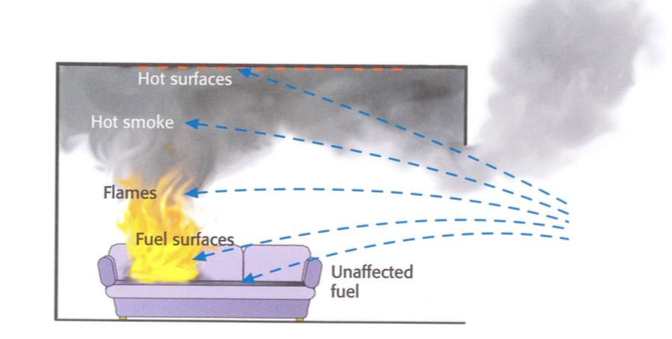
\includegraphics[width=.8\columnwidth]{Figures/Water_Distribution/water_application}
	\caption[Water Application Options]{Water application options. Image from S{\"a}rdqvist~\cite{sardqvist:2002}.}
	\label{fig:Water_Application}
\end{figure}


\section*{Hose Streams and Fire Service Nozzles}
The most important tools on the fire ground have always been hose lines and nozzles as these are vital components to a successful fire suppression operation. In addition to making tactical decisions on the method of fire attack, the firefighters engaged in fire suppression operations also have the ability to vary the nozzle used. The Standard for Fire Hose Connections, NFPA 1963, defines two categories of fire service nozzles: spray and straight tip~\cite{NFPA1963}. A spray nozzle is also known as a combination or fog nozzle while straight tip nozzles are commonly referred to as smooth bore nozzles. There are several different types of spray nozzles including constant gallonage, constant pressure, and adjustable gallonage~\cite{FEHandbook}. The construction of a spray nozzle is more complicated than that of a straight tip nozzle. A straight tip nozzle is a tapered pipe connected to a control valve, or ``bail.'' The tapered pipe is sized such that a given diameter at the tip will provide a given flow at a set pressure. A spray nozzle is constructed using a baffle and spring to provide either a constant flow, constant pressure, or both (TFT Nozzle Guide). Both spray and straight tip nozzles have the ability to provide different flows as well as pressures at the nozzle. It is not uncommon to find different hose lines with different nozzles for specific tactics utilized in a given response area. Fire departments base nozzle choices and hand-line set-ups (hose line size, desired nozzle flow, required pressure) on existing knowledge, traditions, and beliefs. Fire service nozzles serve to control water flow, create shape, and provide reach to hose streams~\cite{Essentials6}. A hose stream, or ``fire stream,'' is defined as a pattern of water that is discharged from a nozzle and travels to a desired target. Spray nozzles can be manually adjusted from a straight stream to a narrow fog to a wide fog as a given tactic requires while straight tip nozzles are limited to a solid stream. Firefighter training literature defines advantages and disadvantages for both types of nozzles as well as the type of hose stream; however, a given nozzle or hose stream is not tied to a specific tactic. These choices are left up to the firefighters engaged in fire suppression operations who must be well informed on the implications of a given tactic and tool.

Whether a fire attack crew chooses to apply water as part of an interior or exterior attack and regardless of the type of nozzle and hose stream chosen, they need to know what impact their stream has on the fire environment ahead of them. This is difficult on the fire ground because visibility is commonly limited and therefore most experience and first-hand accounts are from behind the nozzle. This results in beliefs about conditions (i.e. temperature) ahead of the nozzle team and the impact of their tactics on victim survivability; but knowledge of the actual impact has yet been researched. Additionally, when the fire is ultimately suppressed, there is no assurance the attack was conducted in the most effective, efficient, and safe manner even if the experience gained suggests that it was. Fire service adages such as ``don't put water on smoke,'' ``you will steam the victims,'' and ``fog nozzles always disrupt the thermal layer'' have been passed on from generation to generation with little context or substantiation. Without the context, these concepts get treated like rules and can severely limit firefighters understanding of fire suppression.

The fire attack study is intended to close the knowledge gap and provide both context and substantiation to fire suppression methods, tools, and tactics that have been utilized for decades. The results from this study will provide the fire service with scientific based knowledge on the impact of both interior and exterior fire attack on victim survivability and firefighter safety. Part I of the study, examining water mapping in structures, is the first of two series of experiments looking at the mechanics of hose streams without the presence of fire. The is intended to provide the fire service with a knowledge base into how nozzles distribute water via different hose stream types, nozzle movements, and attack locations in addition to quantifying how nozzles entrain and move air throughout a structure. By developing data in realistic structures utilizing modern fuel sources and fire scenarios, important inferences may be developed relative to different nozzles, hose stream types, techniques, and the overall use of water for fire suppression operations.

\chapter{Objectives and Limitations}

The purpose of this part to the overall study was to provide scientific knowledge on the variation of water flow rate per square foot (water flux) as it pertains to fire service hose streams being directed into compartments. This was accomplished with the completion of the following objectives:

\begin{itemize}
	\setlength{\itemindent}{0.25in}
	\item Adapt measurement apparatus common to sprinkler testing for use in hose stream flow quantification.
	\item Quantify repeatability and uncertainty in apparatus.
	\item Measure water flux data distributions in typical residential compartment for common fire service hose stream configurations.
	\item Quantify similarities and differences of water flux distributions over the range of test variables.
	\item Develop and disseminate knowledge of hose streams applied during typical fire attack methods.
	\end{itemize}

The the experiments conducted were intended to develop a fundamental knowledge of water distribution in compartments from fire service hose streams, without the presence of furniture. This knowledge could then be applied to the infinite number of scenarios in which the fire service may be applying water. The stream locations were chosen to achieve this objective while at the same time simulating some common fireground tactics. Due to the limitations of the equipment used and the force resulting from the application of water with common fire service hoses, directing the hose stream at the collection appliance was not possible nor would it produce a reliable and realistic measurement. However, the fundamental knowledge of water dispersion and distribution gained from the experiments can be applied to scenarios where water is directed at the floor. 

\chapter{Water Distribution Experiments}

The goal of the water distribution experiments was to quantify the impact that changing a nozzle, changing flow/pressure, or changing flow position had on water dispersion within a compartment. Eighty-three water flow tests were conducted at the UL Large Fire Laboratory in Northbrook, IL in a purpose built compartment with an attached hallway and movable staircase. Water flow patterns were determined by collecting the water in 48 discrete collection bins.

\section{Experimental Configuration}

\subsection{Test Apparatus}
\label{ADD_discussion}
The main portion of the test compartment had interior (finished) dimensions of 17~ft 4~in. by 11~ft 4~in with an 8~ft ceiling. To account for water collection apparatus the entire compartment was 7~ft 10 7/8~in above the floor of the lab floor (see Figure~\ref{fig:Water_Distribution_Test_Structure_and_ADD_Apparatus}). The overall size of the compartment was designed to reflect that of one found in a typical resident structure but was also bound by the dimensions of the water collection apparatus (Section~\ref{sec:add_instrumentation}). The compartment was wood frame construction with 2~in. by 4~in. studs and track set to 16~in. centers with a interior height measuring 8~ft 1 1/8~in. rough. The walls and ceiling were lined with 1/2~in. durarock cement board atop 1/2~in. plywood. The ceiling joists were 2~in. by 6~in. set to 16~in. on center.

\begin{figure}[!ht]
	\centering
	\includegraphics[width=.8\columnwidth]{Figures/Water_Distribution/Building.jpg}
	\caption[Water Distribution Test Structure and ADD Apparatus]{Water Distribution Test Structure and ADD Apparatus.}
	\label{fig:Water_Distribution_Test_Structure_and_ADD_Apparatus}
\end{figure}

The compartment featured two openings; one doorway measuring 3~ft by 6~ft 8~in. which opened to the interior hallway, and one window measuring 2~ft by 4~ft with a sill height of 3~ft that opened to the exterior of the compartment. A movable staircase and landing was constructed to provide access to either the interior hallway of the compartment or provide a simulation of a first floor window attack. The hallway was 6~ft by 8~ft and the stairway landing was 4~ft by 6~ft 8~in. Detailed dimension drawings of the compartment are included in Figure~\ref{fig:ADD_Top_View}.

\begin{figure}[!ht]
	\centering
	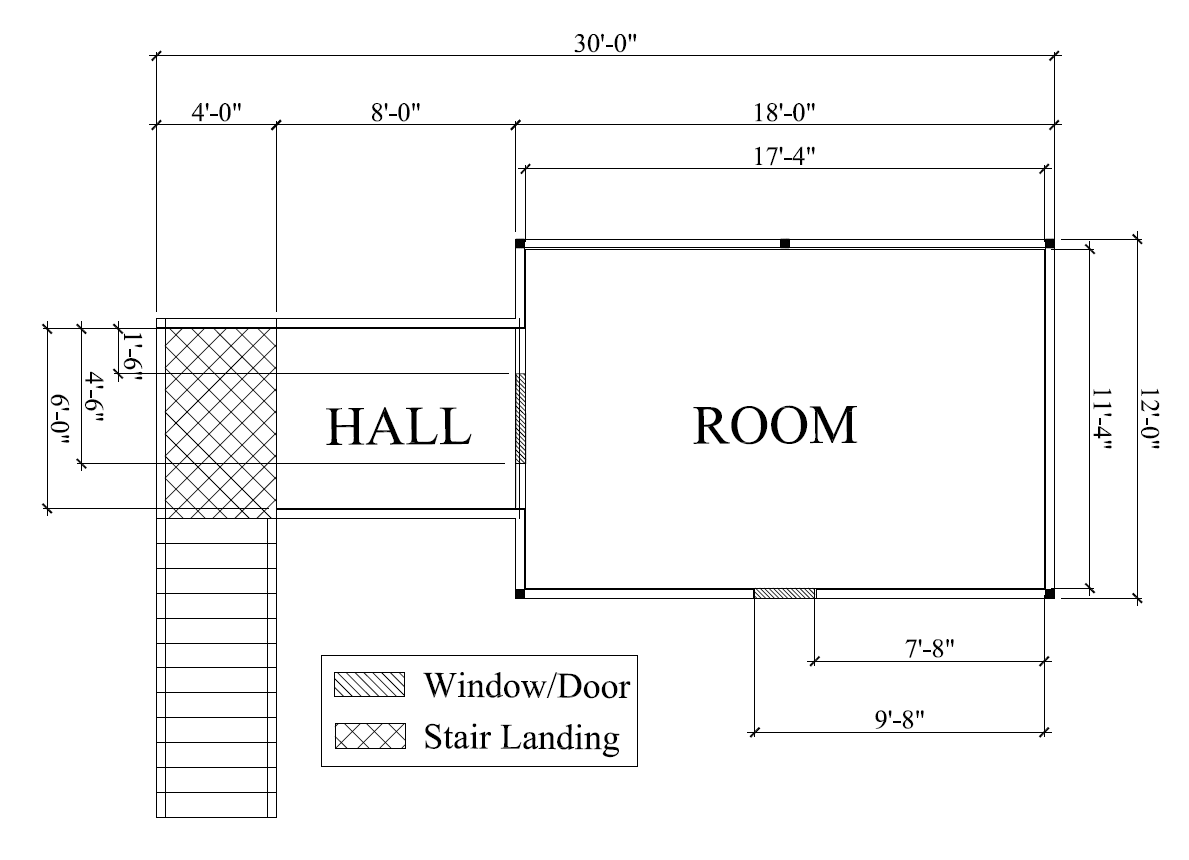
\includegraphics[width=\columnwidth]{Figures/Water_Distribution/ADDtopdownviewtext}
	\caption[Dimensioned Plan View of Experimental Compartment]{Dimensioned plan view of experimental compartment.}
	\label{fig:ADD_Top_View}
\end{figure}

\clearpage

A unique feature of this compartment was that there was no floor constructed. The test compartment instead sat directly over 48, 20~in by 20~in stainless steel collection bins. Instead of water accumulating on the floor, it would flow into the distinct collection bins to determine an accumulation rate. Potential gaps between the collection bins were covered by flashing which was folded to divert the water evenly in each bin, to best ensure adequate distribution results. The gaps between the outer collection bins and the walls of the structure were also covered with flashing to ensure all water directed into the structure was collected in the appropriate bins. The interior layout of the floor bins and use of flashing can be seen in Figure \ref{fig:ADD_Flashing}. 

\begin{figure}[!ht]
	\centering
	\includegraphics[width=.7\columnwidth]{Figures/Water_Distribution/floor3.jpg}
	\caption{Layout of Structure Floor with 48 Collection Bins and Connected Flashing}
	\label{fig:ADD_Flashing}
\end{figure}

\subsection{Instrumentation and Uncertainty}
\label{sec:add_instrumentation}

To measure the water distribution throughout the compartment, a fire sprinkler spray density measurement instrument known as the Actual Delivered Density (ADD) apparatus was used~\cite{Schwille2005}. This device was connected to the 48 collection bins that comprised the floor of the test structure. The ADD apparatus is comprised of one main array and two satellite arrays of heavy steel framework. The main array consists of 32 water barrels and water pan collection assemblies while each satellite array contains 8 barrels and collection assemblies, see Figure~\ref{fig:ADD_Collection_Assembly}. All barrels are of 30-gallon capacity and are connected by a 2~in. diameter hose to a 20~in. by 20~in. inverted square pyramid shaped stainless steel water collection pan above. In total, there are 48 total collection pans/barrels. Differential pressure transducers connect to the bottom of each water collection barrel via flexible tubing. The water level in a given barrel is determined by the head pressure measured by the transducer. The water collection rate is calculated based the change in head pressure over time. As Figure \ref{fig:Bin Numbers and Locations} shows, collection assemblies were arranged into 2~$\times$~2 arrays. Each collection barrel is uniquely numbered so that water flow data can be mapped to specific position. The barrels are connected to a pneumatic drain valve which could be actuated to drain each barrel at the conclusion of an experiment. 

\begin{figure}[!ht]
	\centering
	\begin{tabular}{cc}
		\includegraphics[height = .3\columnwidth]{Figures/Water_Distribution/ADD2.jpg} &
		\includegraphics[height = .3\columnwidth]{Figures/Water_Distribution/ADDbottom3} \\
	\end{tabular}
	\caption[ADD Collection Barrels and Pans]{ADD Collection Barrels (left) and ADD Collection Pans (right).}
	\label{fig:ADD_Collection_Assembly}
\end{figure}

\begin{figure}[!ht]
	\centering
	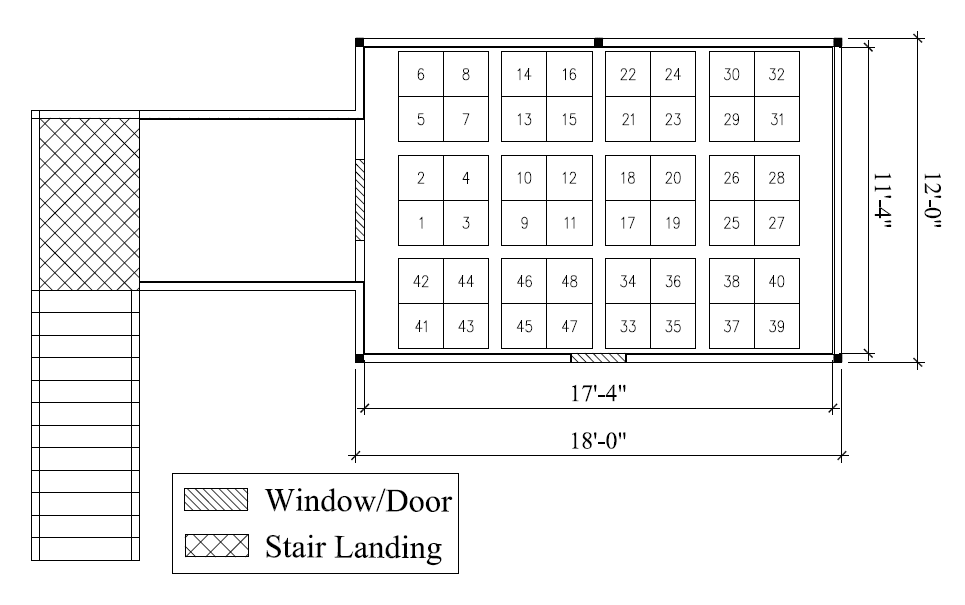
\includegraphics[width=\columnwidth]{Figures/Water_Distribution/ADD_Bins}
	\caption[ADD Bin Numbers and Locations]{Location and numbering of collection bins of ADD apparatus within experimental compartment.}
	\label{fig:Bin Numbers and Locations}
\end{figure}

Prior to testing, data was collected to estimate the uncertainty associated with the water distribution measurements performed using the ADD apparatus. Each water collection assembly was filled to capacity while recording pressure transducer measurements as well as data from a calibrated turbine flowmeter (with less than 1~\% measurement uncertainty). Although the design of each water collection assembly is the same, the measurement performance across the entire apparatus varied. Overall, the 48 water collection assemblies reported an average accuracy of $\pm$ 2.4~gallons. This represents an uncertainty in total volume of $\pm$ 8~\% at full scale (30~gal).

\subsection{Experimental Equipment}

To ensure the data collected were applicable to the majority of the fire service, a representative set of nozzles types, specified flows/pressures, and hose sizes were used which are shown in Table~\ref{tab:nozzles_used_detail}.

\begin{table}[!ht]
\centering
\caption{Primary Equipment Configurations}
\label{tab:nozzles_used_detail}
\begin{tabular}{llccc}
\toprule[1.5pt]
Line Size & Nozzle Type & Tip (in) & Nozzle Pressure (psi) & Approximate Flow Rate (gpm) \\ 
\midrule
1 3/4 in. & Smooth Bore          & 1      & 50 & 210 \\
          & Smooth Bore          & 15/16  & 50 & 185 \\
          & Smooth Bore          & 7/8    & 50 & 160 \\
          & Combination          &        & 100 & 100 \\
          & Combination          &        & 100 & 150 \\
          & Combination          &        & 75 & 150 \\
          & Combination          &        & 50 & 150 \\ \midrule
2 1/2 in. & Smooth Bore          & 1 1/4  & 50 & 325 \\
          & Combination          &        & 100 & 250 \\
\bottomrule[1.25pt]
\end{tabular}
\end{table}

These experiments involved the repetition of nozzle movements and patterns; therefore to minimize nozzle operator fatigue and improve repeatability a nozzle prop was constructed. The prop was used as the `backup' firefighter by supporting the hoseline and minimizing nozzle reaction forces on the operator. Figure~\ref{fig:Nozzle_Prop} shows a dimensioned drawing and the constructed prop. The horizontal base and vertical member were constructed of 4'' by 4'' dimensioned lumber while the angled supports were constructed of 2'' by 6'' dimensioned lumber.

\begin{figure}[!ht]
\centering
    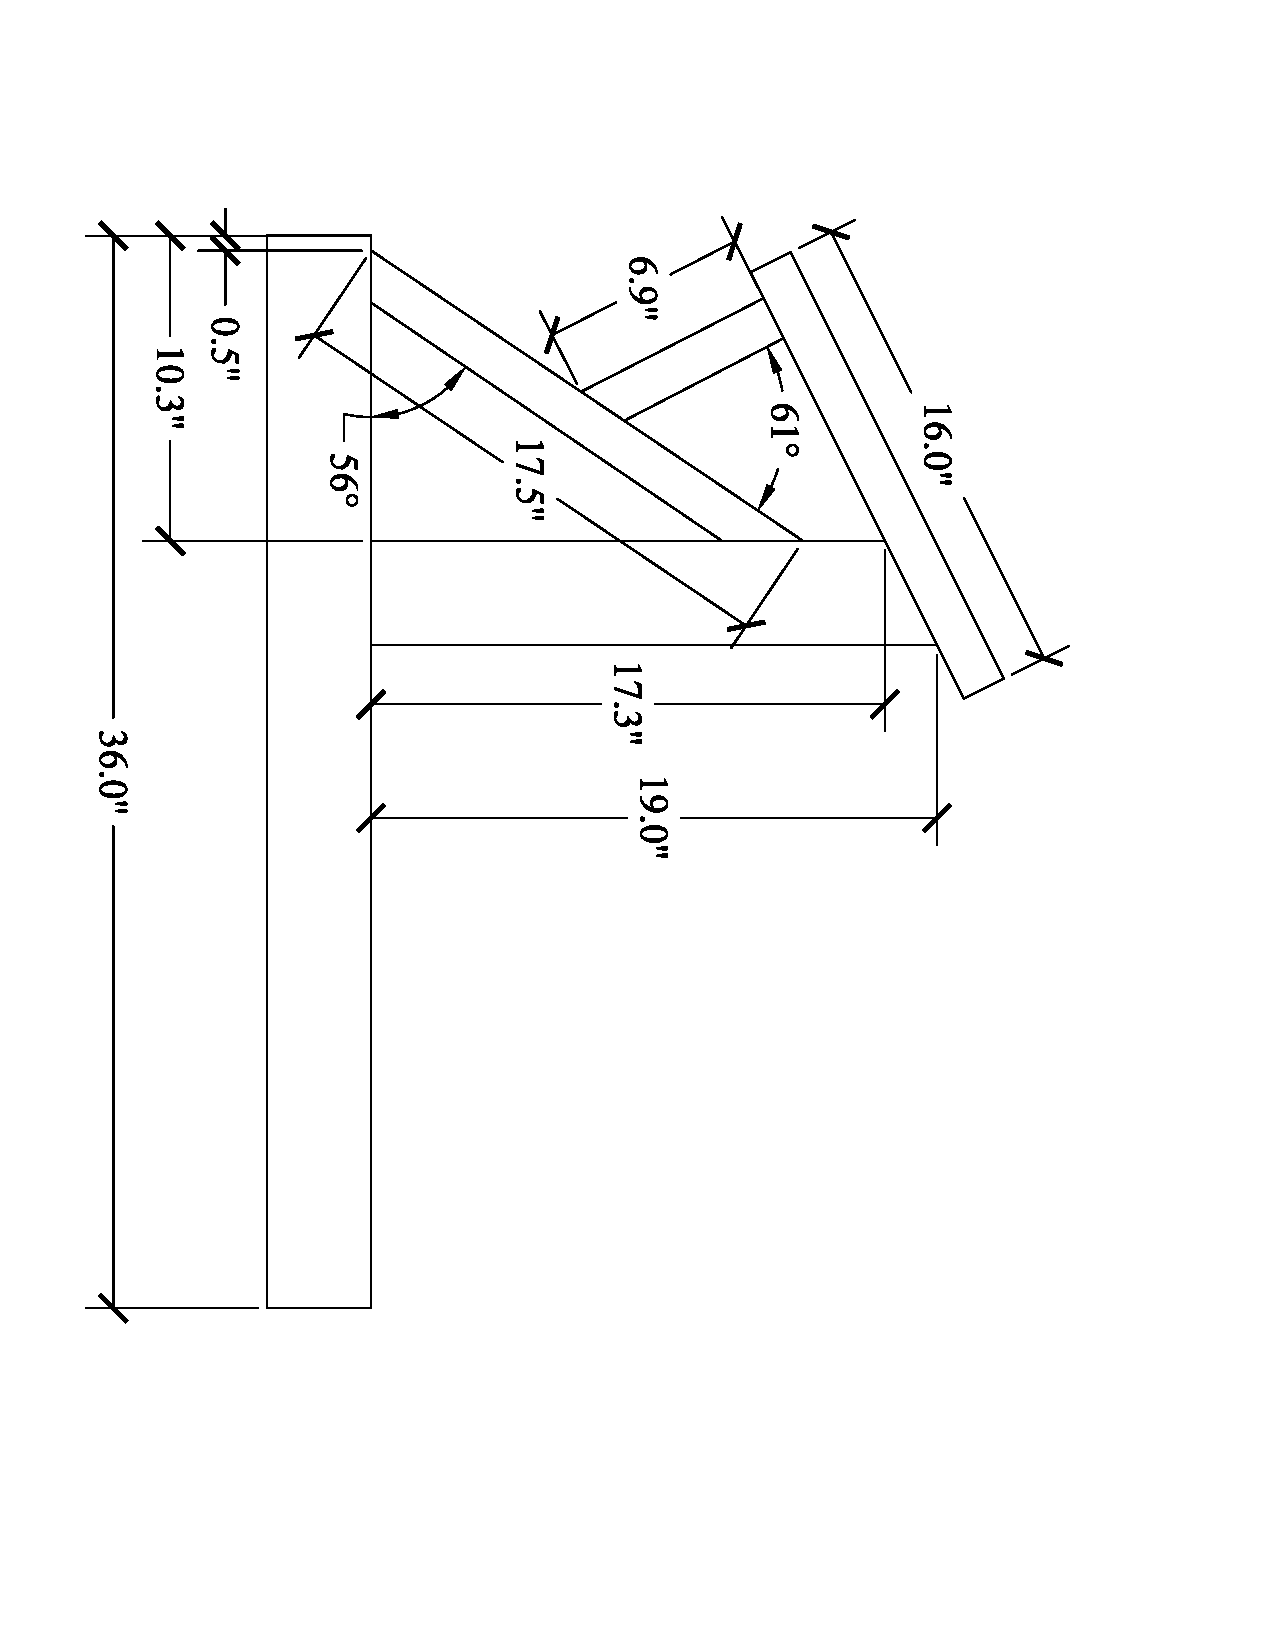
\includegraphics[width=.4\columnwidth]{Figures/Water_Distribution/GIBside}
	\includegraphics[width=.4\columnwidth]{Figures/Air_Entrainment/hoserig}
	\caption[Nozzle Prop]{Dimensioned drawing of the nozzle prop (left) and constructed prop (left).}
	\label{fig:Nozzle_Prop}
\end{figure}

The hose was affixed to the prop with `U' bolts and locking nuts to ensure the hose did not move during an experiment. The prop supported both 1.5~in. and 2.5~in. hoselines. To ensure the experiments were consistent (independent of variance of nozzle position on the prop), the distance from the nozzle to the ventilation opening was measured from the tip of the nozzle, and not the base of the prop.

\begin{figure}[!ht]
\centering
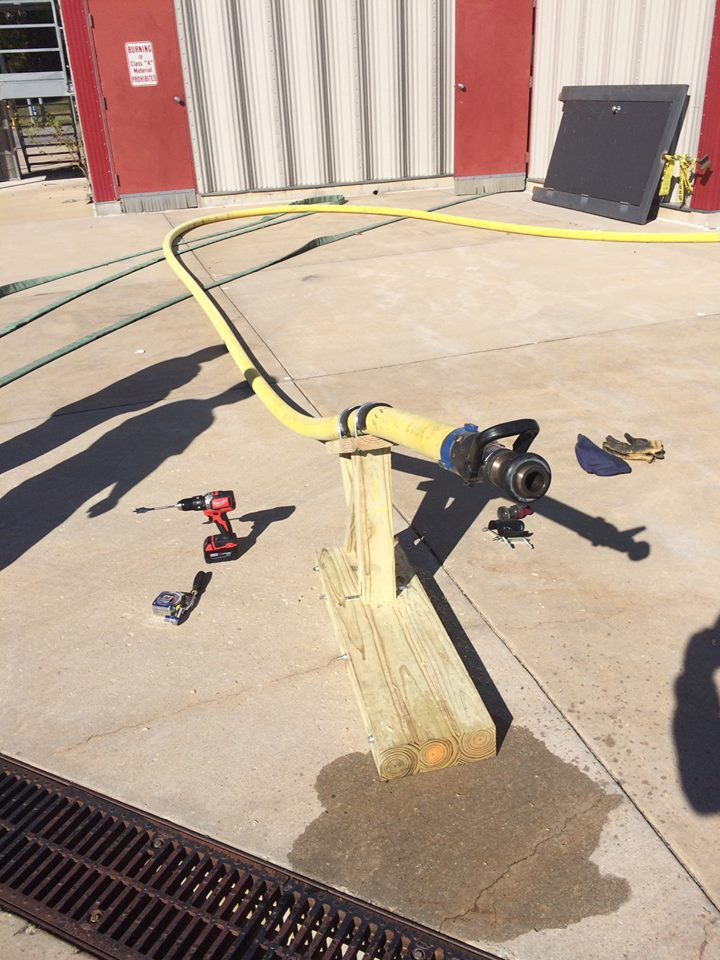
\includegraphics[width=.4\columnwidth]{Figures/Air_Entrainment/Old_Gib} 
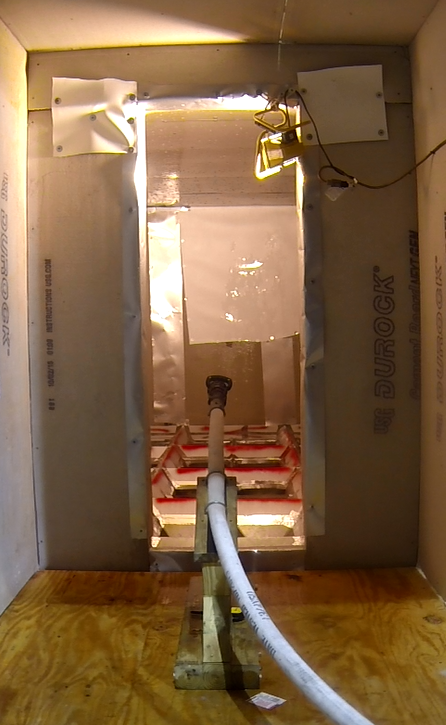
\includegraphics[width=.35\columnwidth]{Figures/Water_Distribution/Nozzle_Directions/Interior_Setup_SS} \\
\caption{Nozzle Prop in Use}
\label{fig:Nozzle_Prop_in_Use}
\end{figure}

\section{Experiments Conducted}

The water distribution experiments consisted of 83 experiments with configuration variables of flow position, doorway or window, nozzle type, pressure at the nozzle, stream angle and stream pattern. In each experiment, water flowed for approximately 1~min. in duration. If a barrel overflowed, there would be an inability to determine the correct distribution of water flow, therefore the duration was dictated by the size of the collection barrels in the ADD apparatus. Each collection barrel was a total of 30~gallons.  At the start of each test, there was an initial amount of water in the bottom of the barrel to ensure the sensors were able to record the water received during the testing. The total water in each barrel was determined by subtracting the initial water volume in each barrel from the final value. The average flux rate was determined by calculating the time average of each barrel over the duration of the flow divided by the effective area of the collection barrel. 

\subsection{Doorway Experiments}
\label{int_tests}
The interior experiments were designed to simulate a fire on the same floor as the attack crew. Suppression operations were conducted from the doorway adjoining the hallway to the test compartment, simulating the location at which an advancing hose crew would cool the fire compartment before entering for final suppression, or the location at an exterior door where water is applied before entry. At this location, hose stream type, nozzle direction, and nozzle movement were varied and the water distribution within the compartment was measured. The three nozzle directions, max angle ceiling, mid ceiling, and at wall are shown in Figure \ref{fig:Nozzle_Direction_Doorway_Attack} and were set from a fixed nozzle location. The max angle ceiling position was defined to be the steepest angle the nozzle could be without the stream being impacted by the soffit of the doorway. The mid ceiling position set the stream to hit the middle of the ceiling along the 14~ft 8~in. dimension. The third position, the wall position, was defined to have the stream hit the vertical midpoint of the wall adjacent to the doorway. Table~\ref{tab:Doorway_Fire_Attack_Distribution_Experiments} lists the interior experiments conducted.

\begin{figure}[!ht]
	\centering
	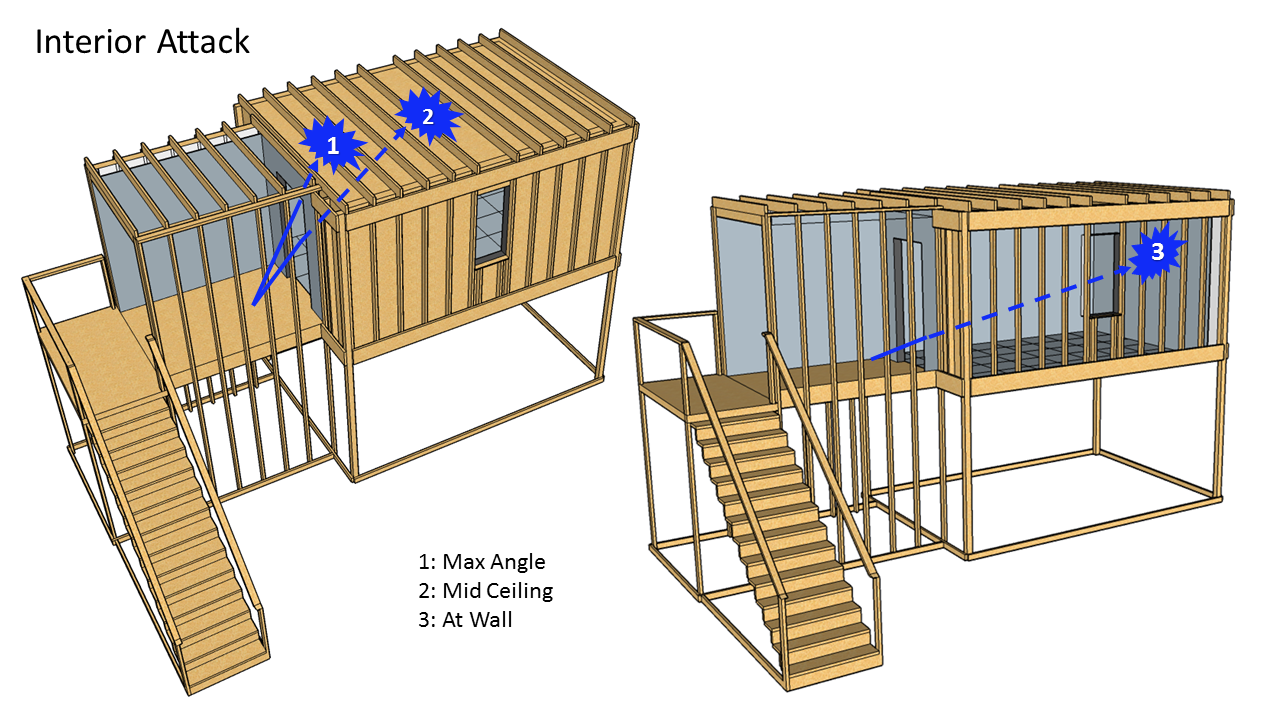
\includegraphics[width=\columnwidth]{Figures/Water_Distribution/Nozzle_Position_Int}
	\caption[Nozzle Direction, Doorway Application]{Nozzle Direction, Doorway Application.}
	\label{fig:Nozzle_Direction_Doorway_Attack}
\end{figure}

\begin{table}[!ht]
\centering
\small
\caption{Doorway Water Distribution Experiments}
\label{tab:Doorway_Fire_Attack_Distribution_Experiments}
\begin{tabular}{ccccc}
\toprule[1.5pt]
Hose Stream Type & Nozzle Direction & Nozzle Movement & Nozzle Pressure (psi) & Rated Flow Rate (gpm) \\ 
\midrule
Straight Stream   & Max Angle Ceiling   & O       & 100 & 150 \\
Straight Stream   & Max Angle Ceiling   & Fixed   & 100 & 150 \\
Straight Stream   & Mid Ceiling 		& Fixed   & 100 & 125 \\
Straight Stream   & Mid Ceiling 		& O       & 100 & 125 \\
Straight Stream   & Mid Ceiling 		& Z       & 100 & 125 \\
Straight Stream   & Mid Ceiling 		& T       & 100 & 125 \\
Straight Stream   & Mid Ceiling 		& Inverted U & 100 & 125 \\
Straight Stream   & Mid Ceiling 		& Fixed   & 100 & 150 \\
Straight Stream   & Mid Ceiling 		& O       & 100 & 150 \\
Straight Stream   & Mid Ceiling 		& Fixed   & 75 & 150 \\
Straight Stream   & Mid Ceiling 		& O & 75  & 150 \\
Straight Stream   & Mid Ceiling 		& Fixed   & 50 & 150 \\
Straight Stream   & Mid Ceiling 		& O & 50  & 150 \\
Straight Stream   & At Wall     		& Fixed   & 100 & 150 \\
Straight Stream   & At Wall     		& O       & 100 & 150 \\
Fog               & Mid Ceiling 		& Fixed   & 100 & 125 \\
Fog               & Mid Ceiling 		& Fixed   & 100 & 150 \\
Fog               & Mid Ceiling 		& O       & 100 & 150 \\
Fog               & Mid Ceiling 		& Fixed   & 75 & 150 \\
Fog               & Mid Ceiling 		& O & 75  & 150 \\
Fog               & Mid Ceiling 		& Fixed   & 50 & 150 \\
Fog               & Mid Ceiling 		& O & 50  & 150 \\
Fog               & Mid Ceiling 		& O       & 100 & 125 \\  
15/16 Smooth Bore & Max Angle Ceiling   & Fixed   & 50 & 180 \\
15/16 Smooth Bore & Max Angle Ceiling   & O & 50  & 180 \\
15/16 Smooth Bore & At Wall     		& Fixed   & 50 & 180 \\
15/16 Smooth Bore & At Wall     		& O & 50  & 180 \\
15/16 Smooth Bore & Mid Ceiling 		& Fixed   & 50 & 180 \\
15/16 Smooth Bore & Mid Ceiling 		& O & 50  & 180 \\
\bottomrule[1.25pt]
\end{tabular}
\end{table}

\clearpage

\subsection{Window Experiments}
\label{ext_tests}

The window experiments included two attack positions; one attack was on grade with fire and the second was when grade was one floor below the fire. These are referred to as first floor and second floor attacks. The movable staircase allowed for the variation between first floor and second floor suppression through the same window vent. The window experiments simulated a single room of fire in which an window attack was used. Similar to the doorway testing, the hose stream type, the nozzle, and nozzle direction were varied for comparison. The differences in first floor and second floor attacks can been seen in Figures \ref{fig:Nozzle_Direction_Window_1st_Floor_Attack} and \ref{fig:Nozzle_Direction_Window_2nd_Floor_Attack}. 

There were five nozzle directions for the first floor window experiments: max angle ceiling, mid ceiling, min angle ceiling, max angle wall, and at wall. The max angle ceiling position was defined as the steepest angle the nozzle could be positioned at without the window soffit impacting the hose stream. The mid ceiling position was defined by the hose stream aimed at the center of the compartment in the 10~ft-5~in dimension. The min angle ceiling position was defined by the shallowest angle such the hose stream did not directly contact the wall. The max angle wall is similar to the max angle ceiling except it was defined as the steepest angle where the hose stream would impact the wall without the stream contacting the ceiling directly. The final position was aiming the stream at the position on the wall across from the window.

There were also five nozzle directions for the second floor window experiments: max angle ceiling, mid ceiling, min angle ceiling, max angle wall, and soffit. The first four positions were the same as the first floor exterior attack except that the starting position of the nozzle changed to be one story below the window vent. The fifth nozzle position, at soffit, was defined to be the maximum angle such that stream directed off the window soffit.

The window experiments are shown in Table~\ref{tab:Window_Fire_Attack_Distribution_Experiments}.

\begin{figure}[!ht]
	\centering
	\includegraphics[width=\columnwidth]{Figures/Water_Distribution/Nozzle_Position_ExtFirstfloor}
	\caption[Nozzle Direction, Window 1st Floor Attack]{Nozzle Direction, Window 1st Floor Attack.}
	\label{fig:Nozzle_Direction_Window_1st_Floor_Attack}
\end{figure}

\begin{figure}[!ht]
	\centering
	\includegraphics[width=\columnwidth]{Figures/Water_Distribution/Nozzle_Position_ExtSecondfloor}
	\caption[Nozzle Direction, Window 2nd Floor Attack]{Nozzle Direction, Window 2nd Floor Attack.}
	\label{fig:Nozzle_Direction_Window_2nd_Floor_Attack}
\end{figure}

\clearpage

\begin{table}[!ht]
\centering
\scriptsize
\caption{Window Water Distribution Experiments}
\label{tab:Window_Fire_Attack_Distribution_Experiments}
\begin{tabular}{lcccccl}
\toprule[1.5pt]
Floor & Hose Stream Type & Nozzle Direction & Nozzle Movement & Nozzle Pressure (psi) & Rated Flow Rate (gpm) & Notes \\ 
\midrule

First  & Straight Stream  & Max Angle Ceiling      & Fixed              & 100 & 150 &   \\
First  & Straight Stream  & Max Angle Ceiling      & Fixed              & 100 & 150 &   \\
First  & Straight Stream  & Max Angle Ceiling      & Fixed              & 100 & 150 &   \\
First  & Straight Stream  & Max Angle Ceiling      & Fixed              & 100 & 150 &   \\
First  & Straight Stream  & Max Angle Ceiling      & Fixed              & 100 & 150 &   \\
First  & Straight Stream  & Max Angle Ceiling      & Fixed              & 100 & 150 &   \\
First  & Straight Stream  & Max Angle Ceiling      & Fixed              & 100 & 150 &   \\
First  & Straight Stream  & Max Angle Ceiling      & Fixed              & 100 & 150 & 1/2 Bale  \\
First  & Straight Stream  & Max Angle Ceiling      & Fixed              & 100 & 150 & 45~s Flow  \\
First  & Straight Stream  & Max Angle Ceiling      & Fixed              & 100 & 150 & 30~s Flow  \\
First  & Straight Stream  & Max Angle Ceiling      & Fixed              & 75  & 150 & 15~s Flow  \\
First  & Straight Stream  & Max Angle Ceiling      & Fixed              & 75  & 60 &   \\
First  & Straight Stream  & Max Angle Ceiling      & Fixed              & 50  & 185 &   \\
First  & Straight Stream  & Max Angle Ceiling      & Fixed              & 50  & 150 &   \\
First  & Straight Stream  & Max Angle Ceiling      & Fixed              & 25  & 150 &   \\
First  & Straight Stream  & Max Angle Ceiling      & Fixed              & 25  & 130 & 30~s Flow  \\
First  & Straight Stream  & Max Angle Ceiling      & Fixed              & 100 & 250 &   \\
First  & Straight Stream  & Max Angle Ceiling      & Sweeping           & 100 & 150 &   \\
First  & Straight Stream  & Max Angle Ceiling      & Wide Sweep         & 100 & 150 &   \\
First  & Straight Stream    & Mid Ceiling          & Fixed      		& 100 & 150 &   \\
First  & Straight Stream    & Min Angle Ceiling    & Fixed     		    & 100 & 150 &   \\
First  & Straight Stream    & Min Angle Ceiling    & Fixed      		& 100 & 250 &   \\
First  & Straight Stream    & Max Angle Wall       & Fixed     		    & 100 & 150 &   \\
First  & Straight Stream    & At Wall              & Fixed      		& 100 & 150 &   \\
First  & 15/16 Smooth Bore  & Max Angle Ceiling      & Fixed         	& 50 & 180 &   \\
First  & 15/16 Smooth Bore  & Max Angle Ceiling      & Sweeping      	& 50 & 180 &   \\
First  & 15/16 Smooth Bore  & Max Angle Ceiling      & Fixed        	& 50 & 180 & 1/2 Bale  \\
First  & 15/16 Smooth Bore  & Max Angle Ceiling      & Fixed        	& 30 & 150 &   \\
First  & 15/16 Smooth Bore  & Max Angle Ceiling      & Fixed        	& 15 & 130 &   \\
First  & 15/16 Smooth Bore  & Max Angle Ceiling      & Fixed        	& 10 & 100 &   \\
First  & 15/16 Smooth Bore  & Mid Ceiling            & Fixed 			& 50 & 180 &   \\
First  & 15/16 Smooth Bore  & Min Angle Ceiling      & Fixed			& 50 & 180 &   \\
First  & 15/16 Smooth Bore  & Max Angle Wall         & Fixed			& 50 & 180 &   \\
First  & 15/16 Smooth Bore  & At Wall                & Fixed 			& 50 & 180 &   \\
First  & 7/8 Smooth Bore    & Max Angle Ceiling      & Fixed         	& 50 & 150 &   \\
First  & 1 Smooth Bore      & Max Angle Ceiling      & Fixed        	& 50 & 210 &   \\
First  & 1 1/4 Smooth Bore  & Max Angle Ceiling      & Fixed         	& 50 & 260 &   \\
First  & Fog                & Max Angle Ceiling      & Fixed        	& 100 & 150 &   \\
First  & Straight Stream/Fog & Max Angle Ceiling    & Fixed/O           & 100 & 150 &   \\
\midrule
Second & Straight Stream    & Max Angle Ceiling      & Fixed                   & 100 & 150 &   \\
Second & Straight Stream    & Max Angle Ceiling      & Sweeping                & 100 & 150 &   \\
Second & Straight Stream    & Max Angle Ceiling      & Wide Sweep              & 100 & 150 &   \\
Second & Straight Stream    & Mid Ceiling            & Fixed                   & 100 & 150 &   \\
Second & Straight Stream    & Min Angle Ceiling      & Fixed                   & 100 & 150 &   \\
Second & Straight Stream    & Max Angle Wall         & Fixed                   & 100 & 150 &   \\
Second & Straight Stream    & Soffit         		 & Fixed                   & 100 & 150 &   \\
Second & 15/16 Smooth Bore  & Max Angle Ceiling      & Fixed                   & 50 & 180 &   \\
Second & 15/16 Smooth Bore  & Max Angle Ceiling      & Sweeping       	       & 50 & 180 &   \\
Second & 15/16 Smooth Bore  & Mid Ceiling            & Fixed                   & 50 & 180 &   \\
Second & 15/16 Smooth Bore  & Min Angle Ceiling      & Fixed                   & 50 & 180 &   \\
Second & 15/16 Smooth Bore  & Max Angle Wall         & Fixed                   & 50 & 180 &   \\
Second & 7/8 Smooth Bore    & Max Angle Ceiling      & Fixed                   & 50 & 150 &   \\
Second & 1 Smooth Bore      & Max Angle Ceiling      & Fixed                   & 50 & 210 &   \\
Second & Fog                & Max Angle Ceiling      & Fixed                   & 100 & 150 & 45~s Flow \\
Second & Fog                & Max Angle Ceiling      & Fixed/O                 & 100 & 150 &   \\
\bottomrule[1.25pt]
\end{tabular}
\end{table}

\chapter{Results}

The intent of the water flow experiments was to determine the distribution of water within the compartment as a function of several common fire service nozzle configurations and application locations. Recall, the location of the water within the compartment was achieved using the ADD device (Section~\ref{sec:add_instrumentation}). 

\section{Repeatability}
\label{sec:repeat}
To ensure that differences between distributions of water flux within the compartment could be quantified, it was important to confirm the repeatability of experiments. The first step was to compare the total volume of water measured in the ADD to the total volume of water expected. Table~\ref{Expected_vs._Experimental_Water_Differences} in Appendix~\ref{app:Water_Volume} shows the expected volume, experimentally measured volume, and percent difference. The average percent different for the experiments was 7.4~\%, within to the expected uncertainty described in Section~\ref{sec:add_instrumentation}. The second step was to compare repeatability between replicate tests. Four experiments utilizing a straight stream pattern from a combination nozzle flowing 150~gpm at 100~psi from a 1 3/4~in. hoseline from the window, first floor position directed into the structure with a maximum angle were conducted to determine the variance in results. The average flux (gpm/ft$^2$) of water in each of the 48 collection bins for the four replicate experiments is shown in Figure~\ref{fig:Repeatability_Testing}. In each the bar chart, bins with less than 0.05 gpm/ft$^2$ are grey, bins that are greater than 0.05~gpm/ft$^2$ but less than 3~gpm/ft$^2$ are colored blue, with more than 3~gpm/ft$^2$ but less than 6~gpm/ft$^2$ are colored green, with more than 6~gpm/ft$^2$ but less than 9~gpm/ft$^2$ are colored yellow, and bins with more than 9~gpm/ft$^2$ are colored red. The choice for the bottom threshold is to provide a relationship to residential sprinklers. According to NFPA 13D, a residential sprinkler system shall provide at least the flow required to produce a minimum discharge density of 0.05~gpm/ft$^2$~\cite{NFPA_13D}.

\begin{figure}[ht]
\begin{tabular*}{\textwidth}{lr}
\includegraphics[width=3.2in]{Script_Figures/ADD_Analysis/15-12-10_082039_Datafile_Rate_Straight_Stream_Window} &
\includegraphics[width=3.2in]{Script_Figures/ADD_Analysis/15-12-10_082423_Datafile_Rate_Straight_Stream_Window} \\
\includegraphics[width=3.2in]{Script_Figures/ADD_Analysis/15-12-10_083305_Datafile_Rate_Straight_Stream_Window} &
\includegraphics[width=3.2in]{Script_Figures/ADD_Analysis/15-12-10_083751_Datafile_Rate_Straight_Stream_Window} \\
\end{tabular*}
\caption[Water Flux for Straight Stream Window at Max Angle]{Water flux in each collection bin for a fixed window straight stream nozzle flowing 150~gpm at 100~psi from the first floor position directed into the structure with a maximum angle. The four bar charts are replicate tests of the same configuration.}
\label{fig:Repeatability_Testing}
\end{figure}

Qualitatively, the array of bars in each chart in Figure~\ref{fig:Repeatability_Testing} look similar to one another. However, to better compare the tests, a statistical approach known as an analysis of variance (ANOVA), was performed. Specifically, the Kruskal-Willis one-way ANOVA test was applied. The goal of this analysis was to quantify whether samples (in this case the flow rate of water in each bin) originate from the same distribution (are the configurations compared similar or different). The Kruskal-Willis analysis was selected because there is no prior assumption that the data is normally distributed. While this statistical analysis can compare $n$ number of data sets and identify if the data sets are statistically different, a limitation in all ANOVAs is the inability to identify which data sets are statistically different. The result of the ANOVA is a p-value. If the p-value is less than 0.05, the experiments being compared are statistically different. If the p-value is large, the experiments being compared are not statistically different.

For the straight stream experiments shown in Figure~\ref{fig:Repeatability_Testing}, a Kruskal-Willis ANOVA test was applied based on average flow rate of water into each collection bin. The resulting p-value was 0.902 average water flux. The high p-value means that the 4 straight stream flow patterns cannot be distinguished from one another. In other words, these experiments can be considered as repeatable.

Confirmation of repeatability, allowed for the exploration of additional comparisons within the data. The main comparison sets examined were variation of hose stream type, variation of nozzle direction, variation of nozzle location, and variation of the flow pressure/flow rate. To best understand the visualization of the water flux distribution plots for the comparison sets, the arrows in Figure~\ref{fig:water_flow} indicate the direction of the flow from the nozzle for doorway tests and window tests.

\begin{figure}[ht]
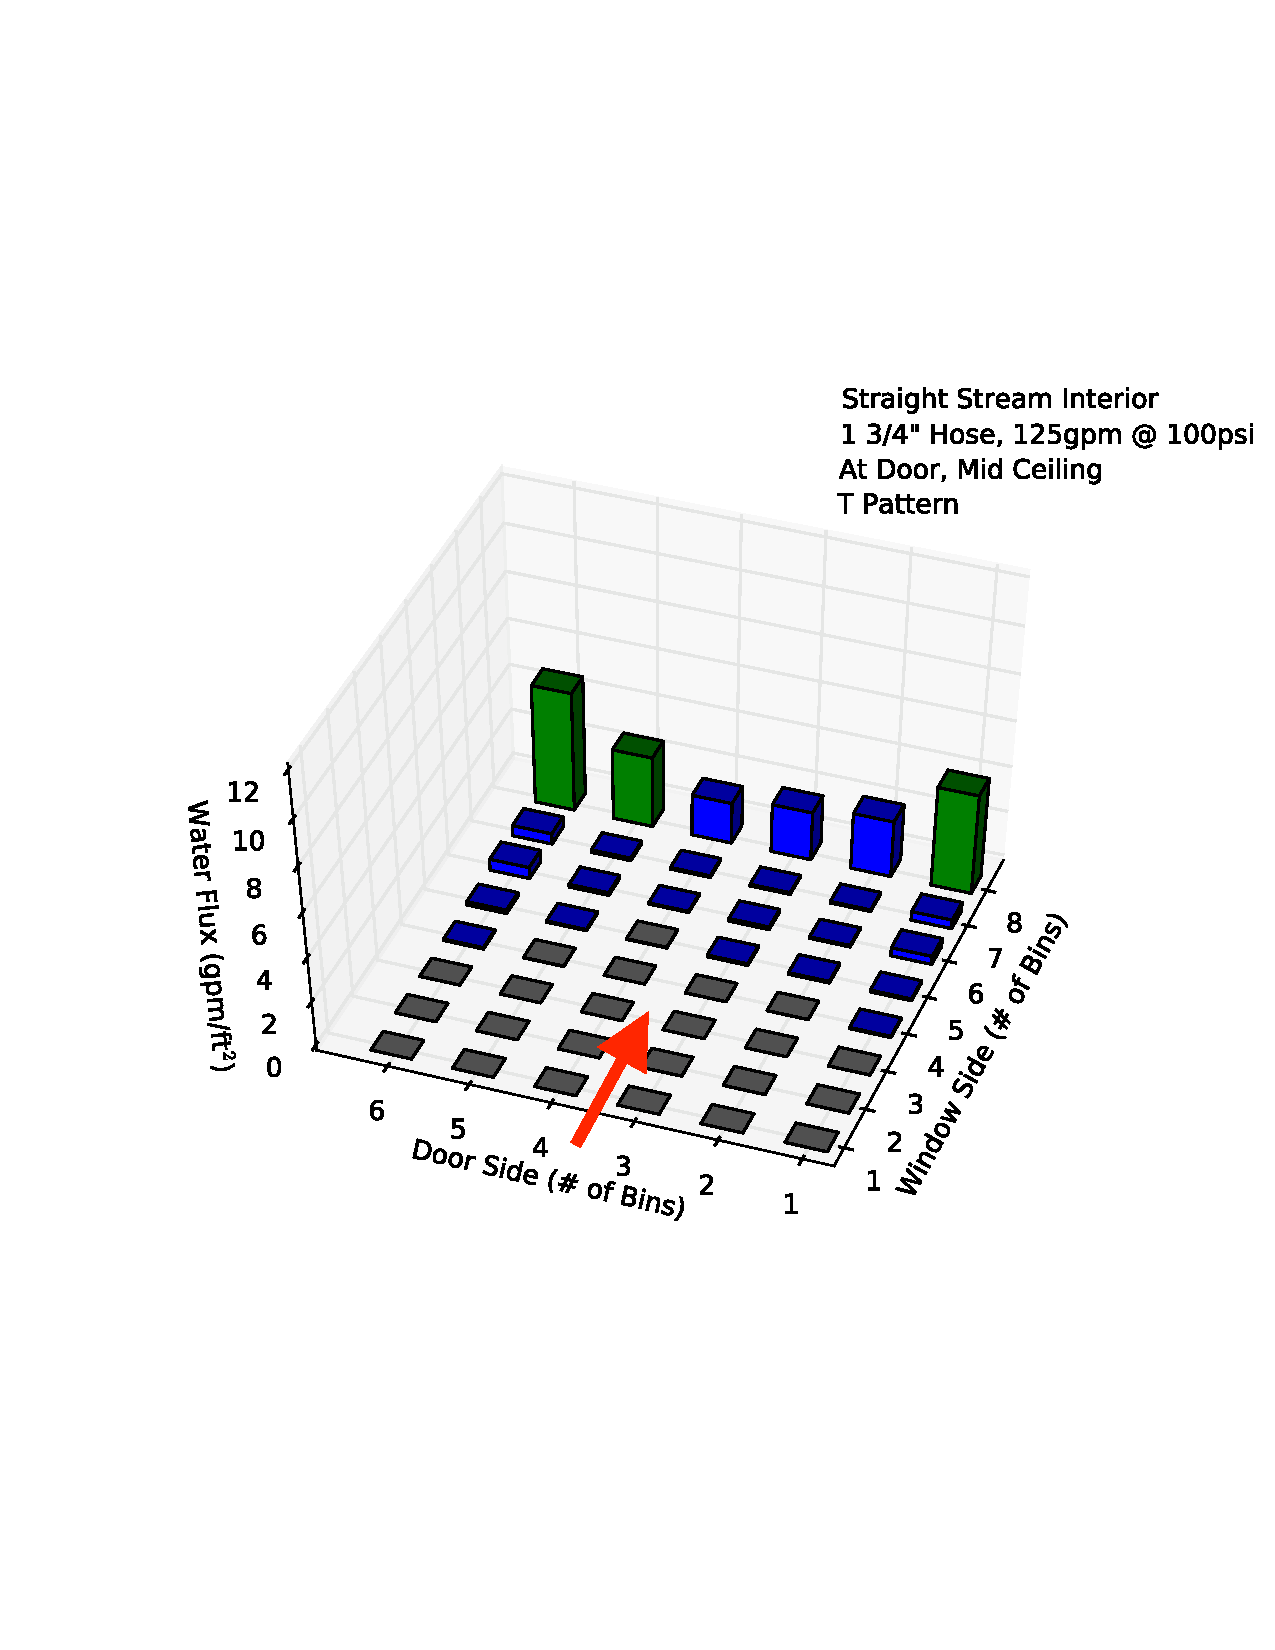
\includegraphics[width=3.2in]{Figures/Water_Distribution/Water_Flux_Interior}
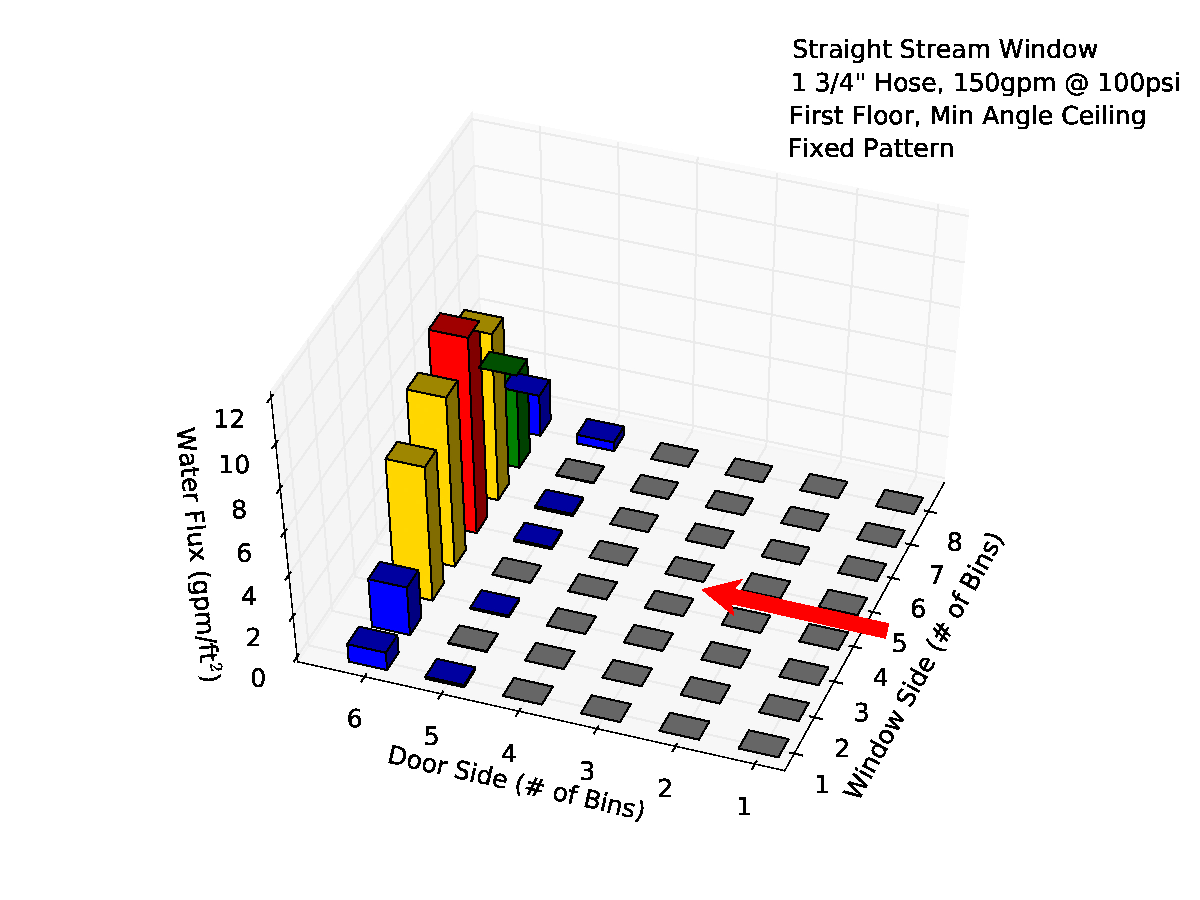
\includegraphics[width=3.2in]{Figures/Water_Distribution/Water_Flux_Exterior}
\caption[Direction of Water Flow on Distribution Plots]{Direction of water flow on distribution plots for doorway experiments (left) and window experiments (right).}
\label{fig:water_flow}
\end{figure}


\section{Comparison of Impact of Hose Stream Type}
\label{sec:streamtype}

The hose stream type experiments were designed to quantify the distributions of water flux from a straight stream, smooth bore stream, and a narrow fog stream. Six configuration sets were analyzed. Within each configuration set, the nozzle direction, nozzle movement, and nozzle pressure/flow rate were fixed. Table~\ref{tab:add_hosestream} shows the results from the ANOVA test based on a comparison of the distribution of the average water flux (gpm/ft$^2$) over the duration of the test within the compartment. The configuration column in the table provides the location (and floor) of the nozzle, the nozzle position, and the nozzle movement. Note that for the window water flow experiments with a sweep pattern, only a straight stream and smooth bore hose stream are compared. The pattern from a fog stream could typically encompass the entire window opening, depending on the size of the opening and the distance from the opening. In these experiments, the fog stream enclosed the window, therefore only a fixed pattern was studied. 

\begin{table}[!ht]
\centering
\small
\caption{Variation of Hose Stream Types: Straight Stream, Smooth Bore Stream, Fog Stream}
\label{tab:add_hosestream}
\begin{tabular}{lccc}
\toprule[1.5pt]
Configuration & \# of Tests & P Value Rate & Different \\ 
\midrule
 Doorway, Mid Ceiling, Fixed Pattern                  & 3          & 2.8E-06 & \checkmark \\
 Doorway, Mid Ceiling, `O' Pattern                    & 3          & 1.0E-04 & \checkmark \\
 1st Floor Window, Max Angle Ceiling, Fixed Pattern  & 3          & 0.050   & \checkmark \\
 2nd Floor Window, Max Angle Ceiling, Fixed Pattern  & 3          & 0.048   & \checkmark \\
 1st Floor Window, Max Angle Ceiling, Sweep Pattern$^*$  & 2      & 0.275   &            \\
 2nd Floor Window, Max Angle Ceiling, Sweep Pattern$^*$  & 2      & 0.501   &            \\
\bottomrule[1.25pt]
$^*$  Only smooth bore stream and straight stream were compared.
\end{tabular}
\end{table}

The results of the statistical analysis identified that 4 of the 6 hose stream comparisons showed statistical difference between the distributions of average water flux. Here, statistical difference means that the resulting distributions likely originated from different sources. In other words, the hose streams that produced the water flux distributions are not the same. For the doorway tests, both the fixed pattern and `O' pattern showed statistical differences (Figures~\ref{fig:Doorway_Varying_Nozzle_Types_Fixed_Pattern} and \ref{fig:Doorway_Varying_Nozzle_Types_O_Pattern}). 

The distributions in Figure~~\ref{fig:Doorway_Varying_Nozzle_Types_Fixed_Pattern} are similar in that the majority of the water flowed into the buckets opposite the doorway and these buckets all had rates greater than a typical residential sprinkler. For the straight stream and smooth bore stream the profile of water flux along the wall in fairly flat. In the case of the fog stream, the flux profile is parabolic with a peak flow at the center and minimums at the corners of the room. For the smooth bore stream, note that along the walls parallel to the flow, there are several buckets that exceed 0.05~gpm/ft$^2$, which the other two hose stream types do not produce. 

Comparison of doorway experiments with the `O' pattern also yielded a p-test value that indicates the streams are different. While the water flux data in Figure~\ref{fig:Doorway_Varying_Nozzle_Types_O_Pattern}, shows increased water coverage within the compartment compared to a fixed stream, there are differences within the hose stream types. The straight stream and fog stream have more pronounced water flux at the corners of the room while the smooth bore steam has a flatter profile. The `O' pattern smooth bore stream has more floor coverage in excess of 0.05~gpm/ft$^2$ especially along the walls parallel to the stream direction.


\begin{figure}[!ht]
\begin{tabular*}{\textwidth}{lr}
\includegraphics[width=3.2in]{Script_Figures/ADD_Analysis/15-12-09_121955_Datafile_Rate_Straight_Stream_Doorway} &
\includegraphics[width=3.2in]{Script_Figures/ADD_Analysis/15-12-09_144839_Datafile_Rate_15_16in_Smooth_Bore_Doorway} \\
\end{tabular*}
\centering
\includegraphics[width=3.2in]{Script_Figures/ADD_Analysis/15-12-09_123142_Datafile_Rate_Fog_Doorway} \\
\caption[Water Flux for Varying Doorway Fixed Pattern Hose Stream Types]{Water flux in each collection bin for doorway fixed pattern flow at the mid-ceiling direction for a straight stream (upper left), smooth bore stream (upper right), and fog stream (bottom middle).}
\label{fig:Doorway_Varying_Nozzle_Types_Fixed_Pattern}
\end{figure}

\begin{figure}[ht]
\begin{tabular*}{\textwidth}{lr}
\includegraphics[width=3.2in]{Script_Figures/ADD_Analysis/15-12-09_122551_Datafile_Rate_Straight_Stream_Doorway} &
\includegraphics[width=3.2in]{Script_Figures/ADD_Analysis/15-12-09_145534_Datafile_Rate_15_16in_Smooth_Bore_Doorway} \\
\end{tabular*}
\centering
\includegraphics[width=3.2in]{Script_Figures/ADD_Analysis/15-12-09_123636_Datafile_Rate_Fog_Doorway}
\caption[Water Flux for Varying Doorway `O' Pattern Hose Stream Types]{Water volume in each collection bin for doorway `O' pattern flow at the mid-ceiling direction for a straight stream (upper left), smooth bore stream (upper right), and fog stream (bottom middle).}
\label{fig:Doorway_Varying_Nozzle_Types_O_Pattern}
\end{figure}

\clearpage

Statistical tests of fixed pattern window experiments for first and second floor locations comparing hose stream types, indicated that both sets showed statistical difference. The p-test values of 0.050 and 0.048  for the first and second floor respectively, indicate that the flux data are different for the straight stream, smooth bore stream and fog stream. For the first floor experiments, the straight stream and smooth bore show more flow around the perimeter of the compartment compared to the fog stream (Figure~\ref{fig:Window_FirstFloor_Fixed_Varying_Nozzle}).

The second floor window experiments examining straight stream, smooth bore stream, and fog stream resulted in a p-value that indicated the hose stream types produced different water flux distributions. Figure~\ref{fig:Window_SecondFloor_Fixed_Varying_Nozzle} shows the flux distributions for the three hose stream types. The straight stream and smooth bore stream show similar flows with a flat profile along the wall opposite the window and values all above the 0.05~gpm/ft$^2$ residential sprinkler threshold, the fog stream produced a noticeably different pattern. The fog stream shows a parabolic pattern along the wall opposite the window and significantly less water flow around the perimeter of the compartment. 

\begin{figure}[ht]
\begin{tabular*}{\textwidth}{lr}
\includegraphics[width=3.2in]{Script_Figures/ADD_Analysis/15-12-08_113237_Datafile_Rate_Straight_Stream_Window} &
\includegraphics[width=3.2in]{Script_Figures/ADD_Analysis/15-12-08_101028_Datafile_Rate_15_16in_Smooth_Bore_Window} \\
\end{tabular*}
\centering
\includegraphics[width=3.2in]{Script_Figures/ADD_Analysis/15-12-08_121806_Datafile_Rate_Fog_Window}
\caption[Water Flux for Varying Window First Floor Fixed Pattern Hose Stream Types]{Water flux in each collection bin for window first floor fixed pattern flow at the max angle direction for a straight stream (upper left), smooth bore stream (upper right), and fog stream (bottom middle).}
\label{fig:Window_FirstFloor_Fixed_Varying_Nozzle}
\end{figure}

\begin{figure}[ht]
\begin{tabular*}{\textwidth}{lr}
\includegraphics[width=3.2in]{Script_Figures/ADD_Analysis/15-12-07_145156_Datafile_Rate_Straight_Stream_Window} &
\includegraphics[width=3.2in]{Script_Figures/ADD_Analysis/15-12-07_111118_Datafile_Rate_15_16in_Smooth_Bore_Window} \\
\end{tabular*}
\centering
\includegraphics[width=3.2in]{Script_Figures/ADD_Analysis/15-12-07_155751_Datafile_Rate_Fog_Window}
\caption[Water Flux for Varying Window Second Floor Fixed Pattern Hose Stream Types]{Water volume in each collection bin for window second floor fixed pattern flow at the max angle direction for a straight stream (upper left), smooth bore stream (upper right), and fog stream (bottom middle).}
\label{fig:Window_SecondFloor_Fixed_Varying_Nozzle}
\end{figure}

\clearpage

The final two comparison sets were both window streams (one first floor set and one second floor set) at the max angle on the ceiling with sweeping patterns. Only the straight stream and smooth bore streams were compared for cases where the nozzle pattern was a sweeping motion from an window position. In both cases, the first floor and second floor location, the analysis revealed that the straight stream and smooth bore stream produce statistically similar distributions. Figures~\ref{fig:Window_FirstFloor_O_Varying_Nozzle} and \ref{fig:Window_SecondFloor_O_Varying_Nozzle} confirm the similarity in the water flux distributions.

\begin{figure}[ht]
\begin{tabular*}{\textwidth}{lr}
\includegraphics[width=3.2in]{Script_Figures/ADD_Analysis/15-12-08_113716_Datafile_Rate_Straight_Stream_Window} &
\includegraphics[width=3.2in]{Script_Figures/ADD_Analysis/15-12-08_101825_Datafile_Rate_15_16in_Smooth_Bore_Window}
\end{tabular*}
\caption[Water Flux for Varying Window First Floor Sweeping Pattern Hose Stream Types]{Water flux in each collection bin for window first floor sweeping pattern flow at the max angle direction for a straight stream (left) and smooth bore stream (right).}
\label{fig:Window_FirstFloor_O_Varying_Nozzle}
\end{figure}

\begin{figure}[ht]
\begin{tabular*}{\textwidth}{lr}
\includegraphics[width=3.2in]{Script_Figures/ADD_Analysis/15-12-07_145842_Datafile_Rate_Straight_Stream_Window} &
\includegraphics[width=3.2in]{Script_Figures/ADD_Analysis/15-12-07_121014_Datafile_Rate_15_16in_Smooth_Bore_Window}
\end{tabular*}
\caption[Water Flux for Varying Window Second Floor Sweeping Pattern Hose Stream Types]{Water volume in each collection bin for window second floor sweeping pattern flow at the max angle direction for a straight stream (left) and smooth bore stream (right).}
\label{fig:Window_SecondFloor_O_Varying_Nozzle}
\end{figure}


\section{Comparison of Impact of Nozzle Direction}
\label{sec:direction}

The second comparison was to quantify the impact of nozzle direction on water distribution within the compartment. Referring back to Figures~\ref{fig:Nozzle_Direction_Doorway_Attack}, \ref{fig:Nozzle_Direction_Window_1st_Floor_Attack}, and \ref{fig:Nozzle_Direction_Window_2nd_Floor_Attack} there are 3, 5, and 5 nozzle directions for the doorway experiments, the window first floor experiments, and the window second floor experiments, respectively. Table~\ref{tab:add_nozzleposition} shows the p-test values comparing average water flux per collection bin  for the nozzle direction comparison experiments.  In all comparisons where the nozzle location was fixed and the nozzle direction was varied, there was sufficient variation in the water flux data to indicate that the data was statistically different. 

\begin{table}[!ht]
\centering
\small
\caption{Variation of Nozzle Directions}
\label{tab:add_nozzleposition}
\begin{tabular}{lccc}
\toprule[1.5pt]
Configuration & \# of Tests & P Value Rate & Different \\ 
\midrule
 Doorway, Smooth Bore, Fixed Pattern                 & 3          & 1.4E-04 & \checkmark  \\
 Doorway, Straight Stream, Fixed Pattern             & 3          & 2.9E-08 & \checkmark  \\
 Doorway, Smooth Bore, `O' Pattern                   & 3          & 2.3E-04 & \checkmark  \\
 Doorway, Straight Stream, `O' Pattern               & 3          & 5.8E-04 & \checkmark  \\
 1st Floor Window, Straight Stream, Fixed Pattern    & 5          & 1.1E-07 & \checkmark  \\
 1st Floor Window, Smooth Bore Fixed Pattern         & 5          & 6.2E-07 & \checkmark  \\
 2nd Floor Window, Straight Stream Fixed Pattern     & 5          & 2.9E-09 & \checkmark  \\
 2nd Floor Window, Smooth Bore Fixed Pattern         & 4          & 1.2E-05 & \checkmark  \\
 1st and 2nd Floor, Window, Straight Stream          & 2          & 0.133   &             \\
\bottomrule[1.25pt]
\end{tabular}
\end{table}

For the doorway tests, there were three nozzle directions examined: max angle ceiling, mid ceiling, and at wall (Figure~\ref{fig:Nozzle_Direction_Doorway_Attack}). The fixed pattern doorway smooth bore stream and straight stream tests both show variation in the data (Table~\ref{tab:add_nozzleposition}) which is also visualized in the water flux charts, Figures~\ref{fig:Doorway_Varying_Nozzle_Direction_SB_Fixed_Pattern} and \ref{fig:Doorway_Varying_Nozzle_Direction_SS_Fixed_Pattern} respectively. Specifically, the max angle ceiling direction for both hose stream types resulted in the perimeter of the compartment exceeding the 0.05~gpm/ft$^2$ water flux of residential sprinklers. At the mid ceiling and wall positions, the water flow is more localized along the wall opposite the doorway.

The doorway `O' pattern smooth bore stream and straight stream experiments were similar to the fixed pattern, Figures~\ref{fig:Doorway_Varying_Nozzle_Direction_SB_O_Pattern} and \ref{fig:Doorway_Varying_Nozzle_Direction_SS_O_Pattern}, respectively. For both hose stream types, moving the nozzle through the three directions resulted in statistically different water flux distributions. Again, the mid ceiling and wall direction showed water concentrated along the wall opposite the doorway while the max angle showed water distributed around the perimeter. 

\begin{figure}[ht]
\begin{tabular*}{\textwidth}{lr}
\includegraphics[width=3.2in]{Script_Figures/ADD_Analysis/15-12-09_145932_Datafile_Rate_15_16in_Smooth_Bore_Doorway} &
\includegraphics[width=3.2in]{Script_Figures/ADD_Analysis/15-12-09_144839_Datafile_Rate_15_16in_Smooth_Bore_Doorway} \\
\end{tabular*}
\centering
\includegraphics[width=3.2in]{Script_Figures/ADD_Analysis/15-12-09_142948_Datafile_Rate_15_16in_Smooth_Bore_Doorway}
\caption[Water Flux for Varying Nozzle Direction with Fixed Doorway Smooth Bore Stream]{Water flux in each collection bin for an doorway smooth bore stream with a fixed pattern at three nozzle directions: max angle ceiling (top left), mid ceiling (top right) and at wall (bottom).}
\label{fig:Doorway_Varying_Nozzle_Direction_SB_Fixed_Pattern}
\end{figure}

\begin{figure}[ht]
\begin{tabular*}{\textwidth}{lr}
\includegraphics[width=3.2in]{Script_Figures/ADD_Analysis/15-12-09_152435_Datafile_Rate_Straight_Stream_Doorway} &
\includegraphics[width=3.2in]{Script_Figures/ADD_Analysis/15-12-09_112850_Datafile_Rate_Straight_Stream_Doorway} \\
\end{tabular*}
\centering
\includegraphics[width=3.2in]{Script_Figures/ADD_Analysis/15-12-09_151401_Datafile_Rate_Straight_Stream_Doorway} 
\caption[Water Flux for Varying Nozzle Direction with Fixed Doorway Straight Stream]{Water flux in each collection bin for an doorway straight stream with a fixed pattern at three nozzle directions: max angle ceiling (top left), mid ceiling (top right) and at wall (bottom).}
\label{fig:Doorway_Varying_Nozzle_Direction_SS_Fixed_Pattern}
\end{figure}

\begin{figure}[ht]
\begin{tabular*}{\textwidth}{lr}
\includegraphics[width=3.2in]{Script_Figures/ADD_Analysis/15-12-09_150300_Datafile_Rate_15_16in_Smooth_Bore_Doorway} &
\includegraphics[width=3.2in]{Script_Figures/ADD_Analysis/15-12-09_145534_Datafile_Rate_15_16in_Smooth_Bore_Doorway} \\
\end{tabular*}
\centering
\includegraphics[width=3.2in]{Script_Figures/ADD_Analysis/15-12-09_144524_Datafile_Rate_15_16in_Smooth_Bore_Doorway}
\caption[Water Flux for Varying Nozzle Direction with `O' Pattern Doorway Smooth Bore Stream]{Water flux in each collection bin for an Doorway smooth bore stream with an `O' pattern at three nozzle directions: max angle ceiling (top left), mid ceiling (top right) and at wall (bottom).}
\label{fig:Doorway_Varying_Nozzle_Direction_SB_O_Pattern}
\end{figure}

\begin{figure}[ht]
\begin{tabular*}{\textwidth}{lr}
\includegraphics[width=3.2in]{Script_Figures/ADD_Analysis/15-12-09_153038_Datafile_Rate_Straight_Stream_Doorway} &
\includegraphics[width=3.2in]{Script_Figures/ADD_Analysis/15-12-09_113335_Datafile_Rate_Straight_Stream_Doorway} \\
\end{tabular*}
\centering
\includegraphics[width=3.2in]{Script_Figures/ADD_Analysis/15-12-09_151823_Datafile_Rate_Straight_Stream_Doorway}
\caption[Water Flux for Varying Nozzle Direction with `O' Doorway Straight Stream]{Water volume in each collection bin for an doorway straight stream with an 'O' pattern at three nozzle directions: max angle ceiling (top left), mid ceiling (top right) and at wall (bottom).}
\label{fig:Doorway_Varying_Nozzle_Direction_SS_O_Pattern}
\end{figure}

\clearpage

The first floor windo experiments used 5 different nozzle directions: max angle ceiling, mid ceiling, min angle ceiling, max angle wall, and at wall. Statistical analysis indicated that the water flux distributions produced from the 5 nozzle direction are not the same for both the smooth bore stream and straight stream experiments. Figure~\ref{fig:Window_First_Floor_Varying_Nozzle_Directions_SB_Fixed_Pattern} shows the water flux distribution for the 5 directions for the smooth bore stream while Figure~\ref{fig:Window_First_Floor_Varying_Nozzle_Directions_SS_Fixed_Pattern} shows the water volume distributions for the straight stream. For both hose stream types, the mid ceiling and min angle ceiling directions indicate that the majority of the water accumulated in the bins along the wall opposite the window. When the direction became steeper (max angle ceiling) the water was distributed around the perimeter, similar to the doorway experiments. When the direction was at the two wall positions a broader distribution occurred. Comparable to the other directions there was still significant flow along the wall opposite the nozzle, but the two ceiling positions showed a broader distribution of water flow, specifically towards window where the nozzle was positioned.

The smooth bore and straight stream second floor window experiments were similar to the first floor window experiments. Changes in nozzle position produced water flux data that was statistically different. Figure~\ref{fig:Window_Second_Floor_Varying_Nozzle_Directions_SB_Fixed_Pattern} shows the results of the water flux distributions for 4 smooth bore directions and \ref{fig:Window_Second_Floor_Varying_Nozzle_Directions_SS_Fixed_Pattern} shows the results of the water flux distributions for 5 straight stream directions. The smooth bore stream max angle ceiling and max angle wall showed the largest spread of water flux, however with different patterns. The max angle ceiling showed a perimeter biased distribution (much like the doorway and fire floor window max angle distributions) while the max angle wall had flux greater than 0.05~gpm/ft$^2$ over two thirds the rows of the collection buckets with the majority of the flow in the two rows along the wall opposite the window. The mid ceiling and min angle ceiling both showed concentrated water flows along the wall opposite the window

Second floor straight stream experiments had similar distributions to the smooth bore stream except that a fifth nozzle direction was included. The window straight stream second floor soffit experiment showed the flattest, most disperse distribution of the the nozzle directions tested.

\begin{figure}[ht]
\begin{tabular*}{\textwidth}{lr}
\includegraphics[width=3.2in]{Script_Figures/ADD_Analysis/15-12-08_101028_Datafile_Rate_15_16in_Smooth_Bore_Window} &
\includegraphics[width=3.2in]{Script_Figures/ADD_Analysis/15-12-08_102802_Datafile_Rate_15_16in_Smooth_Bore_Window} \\
\includegraphics[width=3.2in]{Script_Figures/ADD_Analysis/15-12-08_103414_Datafile_Rate_15_16in_Smooth_Bore_Window} &
\includegraphics[width=3.2in]{Script_Figures/ADD_Analysis/15-12-08_104150_Datafile_Rate_15_16in_Smooth_Bore_Window} \\
\end{tabular*}
\centering
\includegraphics[width=3.2in]{Script_Figures/ADD_Analysis/15-12-08_104620_Datafile_Rate_15_16in_Smooth_Bore_Window} \\
\caption[Water Flux for Varying Nozzle Direction with Fixed First Floor Window Smooth Bore Stream]{Water flux in each collection bin for a first floor window smooth bore stream with a fixed pattern at five nozzle directions: max angle ceiling (top left), mid ceiling (top right), min angle ceiling (middle left), min angle at wall (middle right), and at wall (bottom).}
\label{fig:Window_First_Floor_Varying_Nozzle_Directions_SB_Fixed_Pattern}
\end{figure}

\begin{figure}[ht]
\begin{tabular*}{\textwidth}{lr}
\includegraphics[width=3.2in]{Script_Figures/ADD_Analysis/15-12-08_113237_Datafile_Rate_Straight_Stream_Window} &
\includegraphics[width=3.2in]{Script_Figures/ADD_Analysis/15-12-08_114905_Datafile_Rate_Straight_Stream_Window} \\
\includegraphics[width=3.2in]{Script_Figures/ADD_Analysis/15-12-08_120311_Datafile_Rate_Straight_Stream_Window} &
\includegraphics[width=3.2in]{Script_Figures/ADD_Analysis/15-12-08_121011_Datafile_Rate_Straight_Stream_Window} \\
\end{tabular*}
\centering
\includegraphics[width=3.2in]{Script_Figures/ADD_Analysis/15-12-08_121425_Datafile_Rate_Straight_Stream_Window} \\
\caption[Water Flux for Varying Nozzle Direction with Fixed First Floor Window Straight Stream]{Water flux in each collection bin for a first floor window straight stream with a fixed pattern at five nozzle directions: max angle ceiling (top left), mid ceiling (top right), min angle ceiling (middle left), min angle at wall (middle right), and at wall (bottom).}
\label{fig:Window_First_Floor_Varying_Nozzle_Directions_SS_Fixed_Pattern}
\end{figure}

\begin{figure}[ht]
\begin{tabular*}{\textwidth}{lr}
\includegraphics[width=3.2in]{Script_Figures/ADD_Analysis/15-12-07_111118_Datafile_Rate_15_16in_Smooth_Bore_Window} &
\includegraphics[width=3.2in]{Script_Figures/ADD_Analysis/15-12-07_122135_Datafile_Rate_15_16in_Smooth_Bore_Window} \\
\includegraphics[width=3.2in]{Script_Figures/ADD_Analysis/15-12-07_140034_Datafile_Rate_15_16in_Smooth_Bore_Window} &
\includegraphics[width=3.2in]{Script_Figures/ADD_Analysis/15-12-07_141333_Datafile_Rate_15_16in_Smooth_Bore_Window} \\
\end{tabular*}
\caption[Water Flux for Varying Nozzle Direction with Fixed Second Floor Window Smooth Bore Stream]{Water flux in each collection bin for a second floor window smooth bore stream with a fixed pattern at four nozzle directions: max angle ceiling (top left), mid ceiling (top right), min angle ceiling (bottom left), and max angle wall (bottom left)}
\label{fig:Window_Second_Floor_Varying_Nozzle_Directions_SB_Fixed_Pattern}
\end{figure}

\begin{figure}[ht]
\begin{tabular*}{\textwidth}{lr}
\includegraphics[width=3.2in]{Script_Figures/ADD_Analysis/15-12-07_145156_Datafile_Rate_Straight_Stream_Window} &
\includegraphics[width=3.2in]{Script_Figures/ADD_Analysis/15-12-07_151630_Datafile_Rate_Straight_Stream_Window} \\
\includegraphics[width=3.2in]{Script_Figures/ADD_Analysis/15-12-07_152028_Datafile_Rate_Straight_Stream_Window} &
\includegraphics[width=3.2in]{Script_Figures/ADD_Analysis/15-12-07_155226_Datafile_Rate_Straight_Stream_Window} \\
\end{tabular*}
\centering
\includegraphics[width=3.2in]{Script_Figures/ADD_Analysis/15-12-07_151001_Datafile_Rate_Straight_Stream_Window}
\caption[Water Flux for Varying Nozzle Direction with Fixed Second Floor Window Straight Stream]{Water flux in each collection bin for a second floor window straight stream with a fixed pattern at five nozzle directions: max angle ceiling (top left), mid ceiling (top right), min angle ceiling (middle left), max angle wall (middle right), and soffit (bottom).}
\label{fig:Window_Second_Floor_Varying_Nozzle_Directions_SS_Fixed_Pattern}
\end{figure}

\clearpage

\section{Comparison of Impact of Nozzle Location}

For the window experiments where the hose stream type and nozzle direction were the same, but the starting floor was varied (e.g. 1st and 2nd Floor, Window, Straight Stream, Max Angle) the resulting distributions were similar. For the smooth bore stream and straight stream experiments the three nozzle ceiling positions were compared for the first and second floor starting location. Table~\ref{tab:add_nozzlelocation} shows the statistical analysis results for the comparisons.

\begin{table}[!ht]
\centering
\small
\caption{Variation of Nozzle Location}
\label{tab:add_nozzlelocation}
\begin{tabular}{lccc}
\toprule[1.5pt]
Configuration & \# of Tests & P Value Rate & Different \\ 
\midrule
 1st and 2nd Floor, Window, Smooth Bore, Max Angle       & 2          & 0.780   &             \\
 1st and 2nd Floor, Window, Straight Stream, Max Angle   & 2          & 0.133   &             \\
 1st and 2nd Floor, Window, Smooth Bore, Mid Ceiling     & 2          & 0.872   &             \\
 1st and 2nd Floor, Window, Straight Stream, Mid Ceiling & 2          & 0.122   &             \\
 1st and 2nd Floor, Window, Smooth Bore, Min Angle Ceiling     & 2    & 0.168   &             \\
 1st and 2nd Floor, Window, Straight Stream, Min Angle Ceiling & 2    & 0.173   &             \\
\bottomrule[1.25pt]
\end{tabular}
\end{table}

Window straight streams and smooth bore streams, one from the first floor position and one from the second floor position, were compared. In all cases, the stochastic test showed that the water distributions cannot be considered to be different. Figures~\ref{fig:Window_First_Floor_Second_Floor_SS_Max} and \ref{fig:Window_First_Floor_Second_Floor_SB_Max} show the similar water flux distributions for the max angle ceiling. Figures~\ref{fig:Window_First_Floor_Second_Floor_SS_Mid} and \ref{fig:Window_First_Floor_Second_Floor_SB_Mid} show the similar water flux distributions for the mid ceiling for the straight stream and smooth bore stream, respectively. At the min angle ceiling, the statistical analysis shows the water flux distributions were similar for both streams as a function of floor, Figures~\ref{fig:Window_First_Floor_Second_Floor_SS_MAC} and \ref{fig:Window_First_Floor_Second_Floor_SB_MAC}. Note that for both the smooth bore stream and straight stream there were higher fluxes from the first floor position, particularly at the center of the compartment compared to the second floor.

\begin{figure}[ht]
\includegraphics[width=3.2in]{Script_Figures/ADD_Analysis/15-12-08_113237_Datafile_Rate_Straight_Stream_Window}
\includegraphics[width=3.2in]{Script_Figures/ADD_Analysis/15-12-07_145156_Datafile_Rate_Straight_Stream_Window} \\ 
\caption[Water Flux for Straight Stream Max Angle Varying Window Floor]{Water flux in each collection bin for a first floor window straight stream at max angle ceiling (left) and a second floor window straight stream at max angle ceiling(right).}
\label{fig:Window_First_Floor_Second_Floor_SS_Max}
\end{figure}

\begin{figure}[ht]
\includegraphics[width=3.2in]{Script_Figures/ADD_Analysis/15-12-08_101028_Datafile_Rate_15_16in_Smooth_Bore_Window}
\includegraphics[width=3.2in]{Script_Figures/ADD_Analysis/15-12-07_111118_Datafile_Rate_15_16in_Smooth_Bore_Window} \\ 
\caption[Water Flux for Smooth Bore Max Angle Varying Window Floor]{Water flux in each collection bin for a first floor window smooth bore stream at max angle ceiling (left) and a second floor window smooth bore stream at max angle ceiling(right).}
\label{fig:Window_First_Floor_Second_Floor_SB_Max}
\end{figure}

\begin{figure}[ht]
\includegraphics[width=3.2in]{Script_Figures/ADD_Analysis/15-12-08_114905_Datafile_Rate_Straight_Stream_Window}
\includegraphics[width=3.2in]{Script_Figures/ADD_Analysis/15-12-07_151630_Datafile_Rate_Straight_Stream_Window} \\ 
\caption[Water Flux for Straight Stream Mid Ceiling Varying Window Floor]{Water flux in each collection bin for a first floor window straight stream at mid ceiling (left) and a second floor window straight stream at mid ceiling(right).}
\label{fig:Window_First_Floor_Second_Floor_SS_Mid}
\end{figure}

\begin{figure}[ht]
\includegraphics[width=3.2in]{Script_Figures/ADD_Analysis/15-12-08_102802_Datafile_Rate_15_16in_Smooth_Bore_Window}
\includegraphics[width=3.2in]{Script_Figures/ADD_Analysis/15-12-07_122135_Datafile_Rate_15_16in_Smooth_Bore_Window} \\ 
\caption[Water Flux for Smooth Bore Mid Ceiling Varying Window Floor]{Water flux in each collection bin for a first floor window smooth bore stream at mid ceiling (left) and a second floor window smooth bore stream at mid ceiling(right).}
\label{fig:Window_First_Floor_Second_Floor_SB_Mid}
\end{figure}

\begin{figure}[ht]
\includegraphics[width=3.2in]{Script_Figures/ADD_Analysis/15-12-08_120311_Datafile_Rate_Straight_Stream_Window}
\includegraphics[width=3.2in]{Script_Figures/ADD_Analysis/15-12-07_152028_Datafile_Rate_Straight_Stream_Window} \\ 
\caption[Water Flux for Straight Stream Min Angle Ceiling Varying Window Floor]{Water flux in each collection bin for a first floor window straight stream at min angle ceiling (left) and a second floor window straight stream at min angle ceiling(right).}
\label{fig:Window_First_Floor_Second_Floor_SS_MAC}
\end{figure}

\begin{figure}[ht]
\includegraphics[width=3.2in]{Script_Figures/ADD_Analysis/15-12-08_103414_Datafile_Rate_15_16in_Smooth_Bore_Window}
\includegraphics[width=3.2in]{Script_Figures/ADD_Analysis/15-12-07_140034_Datafile_Rate_15_16in_Smooth_Bore_Window} \\ 
\caption[Water Flux for Smooth Bore Min Angle Ceiling Varying Window Floor]{Water flux in each collection bin for a first floor window smooth bore stream at min angle ceiling (left) and a second floor window smooth bore stream at min angle ceiling(right).}
\label{fig:Window_First_Floor_Second_Floor_SB_MAC}
\end{figure}

\clearpage

\section{Comparison of Impact of Pressure and Flow Rate}
\label{sec:pressure}
The third set of analysis was to quantify the impact of nozzle pressure and nozzle flow rate on water distribution within the compartment. Table~\ref{tab:add_pressure} shows the statistical comparison results for water flux distributions. 

\begin{table}[!ht]
\centering
\footnotesize
\caption{Variation of Nozzle Pressure/Flowrate}
\label{tab:add_pressure}
\begin{tabular}{lccc}
\toprule[1.5pt]
Configuration & \# of Tests & P Value Rate & Different \\ 
\midrule
 Doorway, Straight Stream, Mid Ceiling                     & 3   & 0.190   &            \\
 Doorway, Fog Stream, Mid Ceiling                          & 3   & 0.196   &            \\
 1st Floor Window, Smooth Bore, Max Angle Ceiling          & 3   & 0.815   &            \\
 1st Floor Window Smooth Bore, Vary Tip Size               & 3   & 0.255   &            \\
 1st Floor Window, Straight Stream, Varying Pressure Disc  & 3   & 0.211   &            \\
 1st Floor Window, Varying Stream, Varying Hose Diameter   & 2   & 0.523   &            \\
\bottomrule[1.25pt]
\end{tabular}
\end{table}

Three comparisons examined the impact of changing water pressure: on a straight stream (Figure~\ref{fig:Doorway_Varying_Nozzle_Pressure_SS_Fixed_Pattern}), on a fog stream (Figure~\ref{fig:Doorway_Varying_Nozzle_Pressure_Fog_Fixed_Pattern}) and on a smooth bore stream (Figure~\ref{fig:Window_First_Floor_Varying_Nozzle_Pressure_SB_Fixed_Pattern}). For each of these three hose stream types, the statistical analysis of the results of flow rate revealed that varying pressure did not result in distinctly different water flux distributions. The straight stream experiments were conducted at 100~psi, 75~psi, and 50~psi. For all three pressures, the water flux is similar in position (along the wall opposite the door) and profile (cf. Figure~\ref{fig:Doorway_Varying_Nozzle_Pressure_SS_Fixed_Pattern}). The fog nozzle experiments were conducted at the same three pressures as the straight stream: 100~psi, 75~psi, and 50~psi. The distributions, shown in Figure~\ref{fig:Doorway_Varying_Nozzle_Pressure_Fog_Fixed_Pattern}, all have similar parabolic profiles along the wall opposite the doorway. For the smooth bore stream, three flow rates were compared: 180~gpm at 50~psi, 150~gpm at 30~psi, and 130~gpm at 15~psi. In these cases, the total water flowed was decreased with decreased flow rate, but as Figure~\ref{fig:Window_First_Floor_Varying_Nozzle_Pressure_SB_Fixed_Pattern} shows, the distributions are similar although the magnitude of the flux changed.

\begin{figure}[ht]
\begin{tabular*}{\textwidth}{lr}
\includegraphics[width=3.2in]{Script_Figures/ADD_Analysis/15-12-09_112850_Datafile_Rate_Straight_Stream_Doorway} &
\includegraphics[width=3.2in]{Script_Figures/ADD_Analysis/15-12-09_115707_Datafile_Rate_Straight_Stream_Doorway} \\
\end{tabular*}
\centering
\includegraphics[width=3.2in]{Script_Figures/ADD_Analysis/15-12-09_121955_Datafile_Rate_Straight_Stream_Doorway}
\caption[Water Flux Varying Pressure with Straight Stream]{Water flux in each collection bin for an doorway straight stream with a fixed pattern at 150~gpm with 100~psi (top left), 75~psi (top right) and 50~psi (bottom).}
\label{fig:Doorway_Varying_Nozzle_Pressure_SS_Fixed_Pattern}
\end{figure}

\begin{figure}[ht]
\begin{tabular*}{\textwidth}{lr}
\includegraphics[width=3.2in]{Script_Figures/ADD_Analysis/15-12-09_113802_Datafile_Rate_Fog_Doorway} &
\includegraphics[width=3.2in]{Script_Figures/ADD_Analysis/15-12-09_120821_Datafile_Rate_Fog_Doorway} \\
\end{tabular*}
\centering
\includegraphics[width=3.2in]{Script_Figures/ADD_Analysis/15-12-09_123142_Datafile_Rate_Fog_Doorway}
\caption[Water Flux Varying Pressure with Fog Stream]{Water flux in each collection bin for an doorway fog stream with a fixed pattern at 150~gpm with 100~psi (top left), 75~psi (top right) and 50~psi (bottom).}
\label{fig:Doorway_Varying_Nozzle_Pressure_Fog_Fixed_Pattern}
\end{figure}

\begin{figure}[ht]
\begin{tabular*}{\textwidth}{lr}
\includegraphics[width=3.2in]{Script_Figures/ADD_Analysis/15-12-08_101028_Datafile_Rate_15_16in_Smooth_Bore_Window} &
\includegraphics[width=3.2in]{Script_Figures/ADD_Analysis/15-12-08_154306_Datafile_Rate_15_16in_Smooth_Bore_Window} \\
\end{tabular*}
\centering
\includegraphics[width=3.2in]{Script_Figures/ADD_Analysis/15-12-08_154812_Datafile_Rate_15_16in_Smooth_Bore_Window}
\caption[Water Flux Varying Pressure with Smooth Bore Stream]{Water flux in each collection bin for a first floor doorway smooth bore a fixed pattern with 180~gpm at 50~psi (top left), 150~gpm at 30~psi (top right) and 130~gpm at 15~psi (bottom).}
\label{fig:Window_First_Floor_Varying_Nozzle_Pressure_SB_Fixed_Pattern}
\end{figure}

\clearpage

In addition to examining a fixed smooth bore nozzle with varying pressure, three smooth bore nozzles with different sizes were examined. The three configurations were a 1~in. tip that flowed 210~gpm at 50~psi, 15/16~in. tip that flowed 185~gpm at 50~psi, and a 7/8~in. tip that flow 160~gpm at 50~psi. Variation of tip size resulted in water flux distributions that could not be distinguished from one another. Figure~\ref{fig:Window_Second_Floor_Varying_Flow_Rates_SB_Fixed_Pattern} shows the water flux results for the three experiments. The distributions, while similar, do differ in magnitude,

\begin{figure}[ht]
\begin{tabular*}{\textwidth}{lr}
\includegraphics[width=3.2in]{Script_Figures/ADD_Analysis/15-12-07_143828_Datafile_Rate_1in_Smooth_Bore_Window} &
\includegraphics[width=3.2in]{Script_Figures/ADD_Analysis/15-12-07_111118_Datafile_Rate_15_16in_Smooth_Bore_Window} \\
\end{tabular*}
\centering
\includegraphics[width=3.2in]{Script_Figures/ADD_Analysis/15-12-07_143141_Datafile_Rate__7_8in_Smooth_Bore_Window}
\caption[Water Flux Varying Tip Size for Smooth Bore Nozzle]{Water flux in each collection bin for an window smooth bore stream with a fixed pattern with a 1~in. tip (top left), 15/16~in. tip (top right) and 7/8~in. tip (bottom).}
\label{fig:Window_Second_Floor_Varying_Flow_Rates_SB_Fixed_Pattern}
\end{figure}

To compare the impact of changing pressure disc options in a combination nozzle, three first floor window straight stream experiments at the max angle nozzle direction were compared. The three settings were 150~gpm at 100~psi, 185~gpm at 50~psi, and 150~gpm at 50~psi. Figure~\ref{fig:Window_First_Floor_Varying_Nozzle_Pressure_SS_Fixed_Pattern} shows the water flux patterns that are similar to one another, which is confirmed by the statistical analysis indicating the distributions are similar.   

\begin{figure}[ht]
\begin{tabular*}{\textwidth}{lr}
\includegraphics[width=3.2in]{Script_Figures/ADD_Analysis/15-12-08_113237_Datafile_Rate_Straight_Stream_Window} & 
\includegraphics[width=3.2in]{Script_Figures/ADD_Analysis/15-12-08_162126_Datafile_Rate_Straight_Stream_Window} \\
\end{tabular*}
\centering
\includegraphics[width=3.2in]{Script_Figures/ADD_Analysis/15-12-08_160630_Datafile_Rate_Straight_Stream_Window}  
\caption[Water Flux Varying Pressure Discs in Combination Nozzle]{Water flux in each collection bin for a first floor window straight stream with a fixed pattern at 150~gpm at 100~psi (top left), 185~gpm at 50~psi (top right) and 150~gpm at 50~psi (bottom).}
\label{fig:Window_First_Floor_Varying_Nozzle_Pressure_SS_Fixed_Pattern}
\end{figure}

\clearpage

Tests were also conducted to examine if increasing the hose diameter to provide additional water would impact the flux of water within the compartment. A 15/16~in. smooth bore nozzle on a 1 3/4~in. hose provided 180~gpm at 50~psi. The results were compared to those produced by a 1 1/4~in. smooth bore nozzle on a 2 1/2~in. hose which provided 260~gpm at 50~psi. The water flux distributions are shown to be statistically similar, a p-value of 0.523, and Figure~\ref{fig:Window_First_Floor_Varying_Hose_Size} shows that despite a couple bins have greater water flux for the larger hose the distributions are comparable.

\begin{figure}[ht]
\includegraphics[width=3.2in]{Script_Figures/ADD_Analysis/15-12-08_101028_Datafile_Rate_15_16in_Smooth_Bore_Window}
\includegraphics[width=3.2in]{Script_Figures/ADD_Analysis/15-12-08_144238_Datafile_Rate_1_1_4in_Smooth_Bore_Window} \\ 
\caption[Water Flux Varying Hose Size]{Water flux in each collection bin for a first floor window stream with a fixed pattern from 1 3/4~in. straight stream (left) and 2 1/2 in. smooth bore with 1 1/4 in. tip (right).}
\label{fig:Window_First_Floor_Varying_Hose_Size}
\end{figure}

\chapter{Discussion}

\section{Hose Stream Reach}
\label{sec:hose_reach}
There has been research on firefighting nozzles and hose streams as far back as late 1800's~\cite{CHICAGO_TRIBUNE:1339:a}. Limited by available technology at the time, this early work focused on visual observations. Specifically, researchers focused on distance, or effective reach. Effective reach was defined as the reach of the hose stream before it began to break apart. Without the aid of modern personal protective equipment, early fire service nozzles needed to be designed for reach; to provide protection for firefighters by keeping distance between them and the fire. A long reach also meant a greater ability to suppress fires on upper floors without having to drag hoselines through the building. Additionally, the research on adjustable nozzles, which have been in the fire service over 100~years~\cite{PALMER:1878}, has focused on reach, flow, and patterns. 

The second edition of Fire Service Hydraulics by Sylvia, which contains information on the reach of hose streams both vertically and horizontally~\cite{SYLVIA:1970}, cites original work done by John R. Freeman. Mr. Freeman was a civil engineer who conducted tests of hand held nozzle reach in 1884. Results of his work indicated the maximum effective horizontal reach of a $\frac{3}{4}$~in nozzle was achieved when the nozzle was at a 32$^\circ$ angle. Through the data Mr. Freeman collected, an empirical formula was developed for maximum horizontal effective reach ($S$ [ft]) as a function of pressure ($p$ [psi]): 

\begin{equation*}
	S = \frac{1}{2}p+26
\end{equation*}

For nozzles sizes in excess of $\frac{3}{4}$~in add 5 to the 26 for each $\frac{1}{8}$~in increase in nozzle diameter. 

A formula for maximum vertical reach, or effective height, ($H$ [ft]) was also derived from empirical data. For an angle of 70$^{\circ}$ and a 1~in smooth bore tip with a nozzle pressure ($p$ [psi]) up to 100~psi, the effective height can be found from:

\begin{equation*}
	H = \sqrt{240p - p^2 - 1900} -15
\end{equation*}

Over the last 200~yrs little has changed in how nozzle reach is determined. Studies conducted by nozzle manufacturers indicate modern nozzles using a straight stream from a combination nozzle or smooth bore have an effective reach of anywhere from 45~ft to 145~ft, using the same 32$^\circ$ angle from Freeman's work~\cite{TFT_Reach,Elkhart_Reach,Akron_Reach}. Modern combination and smooth bore nozzles are commonly used for interior fire attack of residential structures, however the largest dimension within a room typically on the order of 25~ft. As a result, during an interior attack of a residential structure, the hose stream will likely impact an obstruction before it exceeds its effective reach. Even combination nozzles set to a narrow fog (30$^\circ$) are cited to have an effective reach of 40~ft to 50~ft~\cite{Elkhart_Reach}.

\section{Hose Stream Dispersion}
\label{sec:dispersion}
Quantification of the impact to a hose stream once it impacts a solid obstruction (dispersion) is difficult. Additionally, visual observation gained from experience using hose streams on residential fires is nearly impossible due to smoke within the structure. Work done by the national board of fire underwriters indicates the hose stream velocity to be in excess of 80~ft/s~\cite{NBFU:EffectiveReach}. That velocity, combined with the density of water being 8.3~lb/gal~\cite{SFPEHandbookPurser} results in a water stream with significant momentum. Once the stream impacts a surface, some of the momentum is absorbed (slowing down the stream) while the remainder is transmitted in different directions (redirecting the stream). 

Stream dispersion is dependent on the angle of impact. When the angle of impact was close to 90$^{\circ}$ as shown in Figure~\ref{fig:90DegreeImpact} the stream was redirected radially, approximately in a 360$^{\circ}$ pattern. Note that since this was a horizontal flow (90$^{\circ}$ to a vertical wall), gravity did skew the dispersion downward as the arrows in Figure~\ref{fig:90DegreeImpact} indicate.  

\begin{figure}[!ht]
\centering
\includegraphics[width=0.5\textwidth]{Figures/Water_Distribution/Nozzle_Directions/Exterior_AtWall_SB_Arrows}
\caption[Water Dispersion Straight Stream 90$^{\circ}$ Impact Angle]{Water dispersion of straight stream impacting a wall at an approximate 90$^{\circ}$ angle.}
\label{fig:90DegreeImpact}
\end{figure}

For the cases where the stream was aimed at the ceiling, a 90$^{\circ}$ angle could not have been tested without the nozzle placed being inside the compartment. Therefore, the maximum angle was defined as the angle closest to 90$^{\circ}$ while the nozzle remained exterior (recall Figures~\ref{fig:Nozzle_Direction_Window_1st_Floor_Attack} and \ref{fig:Nozzle_Direction_Window_2nd_Floor_Attack}). Figure~\ref{fig:MaxAngleCeilingImpact} shows the impact on the stream. The majority of the water was directed along the ceiling toward the wall opposite of nozzle. There was some water that was directed back in the direction towards the wall where the nozzle was positioned. Note that water did not ``bounce'' of the ceiling and fall into the center collection bins.

\begin{figure}[!ht]
\centering
\includegraphics[width=0.5\textwidth]{Figures/Water_Distribution/Nozzle_Directions/Exterior_MaxAngleCeiling_SS_Arrows} 
\caption[Water Dispersion Straight Stream Max Angle Ceiling]{Water dispersion of straight stream impacting a ceiling at the maximum angle.}
\label{fig:MaxAngleCeilingImpact}
\end{figure}

As the angle between the stream and ceiling decreased (stream became more parallel to the ceiling), the momentum of the water carried more water towards the wall opposite the nozzle. Figures~\ref{fig:MidCeilingImpact} and \ref{fig:MidCeilingImpact} show the impact of decreasing the angle on the dispersion of water within the compartment for a mid ceiling nozzle direction and min angle ceiling nozzle direction respectively. When the stream impacted the ceiling at an angle, there was limited to no ricochet off the ceiling. The stream dispersed into a fan shape and continued in the direction of travel. Once it struck the back wall, the momentum was translated down the back wall. 

\begin{figure}[!ht]
\centering
\includegraphics[width=0.5\textwidth]{Figures/Water_Distribution/Nozzle_Directions/Exterior_MidCeiling_SS_Arrows}
\caption[Water Dispersion Straight Stream Middle Position Ceiling]{Water dispersion of straight stream impacting a ceiling at the middle position.}
\label{fig:MidCeilingImpact}
\end{figure}

\begin{figure}[!ht]
\centering
\includegraphics[width=0.5\textwidth]{Figures/Water_Distribution/Nozzle_Directions/Exterior_MinAngleCeiling_SS_FirstFloor_Arrows}
\caption[Water Dispersion Straight Stream Minimum Angle Ceiling]{Water dispersion of straight stream impacting a ceiling at the minimum angle.}
\label{fig:MinAngleCeilingImpact}
\end{figure}

Figure \ref{fig:Mid_Ceiling_Dispersion} provides a mid ceiling nozzle position view from the perspective of the collection buckets ``looking'' toward the ceiling for both a smooth bore stream and a straight stream. While the straight stream shows a slightly larger diameter stream before ceiling impact, both streams show similar dispersion patterns after impacting the ceiling. 

\begin{figure}[!ht]
\centering
\centering
\includegraphics[width=0.6\textwidth]{Figures/Water_Distribution/Nozzle_Directions/Exterior_MidCeiling_SB_FirstFloor_Under} \\
\includegraphics[width=0.6\textwidth]{Figures/Water_Distribution/Nozzle_Directions/Exterior_MidCeiling_SS_FirstFloor_Under}
\caption[Water Dispersion for Smooth Bore Stream and Straight Stream at Mid Ceiling]{Dispersion at the  mid ceiling nozzle position from below for a smooth bore stream (top) and straight stream (bottom).}
\label{fig:Mid_Ceiling_Dispersion}
\end{figure}

Although the shape of the stream when it hits the surface has some impact on the dispersion, in general the momentum of the water carries the resulting droplets in the same general direction. For a fog stream that impacted the ceiling, the momentum of the droplets still carried them in the general direction of the stream. As the angle of impact with the surface is decreased as shown in Figure~\ref{fig:MaxAngleCeilingFogImpact} and \ref{fig:MinAngleCeilingFogImpact} the dispersion is similar to the smooth bore stream and straight stream: more directional than radial with the momentum carrying more of the droplets in the original direction of the stream.

\begin{figure}[!ht]
\centering
\includegraphics[width=0.6\textwidth]{Figures/Water_Distribution/Nozzle_Directions/Interior_MaxAngleCeiling_Fog_Arrows}
\caption[Water Dispersion Fog Stream Maximum Angle Ceiling]{Water dispersion of fog stream impacting a ceiling at the maximum angle.}
\label{fig:MaxAngleCeilingFogImpact}
\end{figure}

\begin{figure}[!ht]
\centering
\includegraphics[width=0.6\textwidth]{Figures/Water_Distribution/Nozzle_Directions/Interior_MidCeiling_Fog_Arrows} 
\caption[Water Dispersion Fog Stream Mid Angle Ceiling]{Water dispersion of fog stream impacting a ceiling at the mid angle.}
\label{fig:MinAngleCeilingFogImpact}
\end{figure}


\section{Water Distribution}
\label{sec:water_dist}

If a stream impacts a wall at near a 90$^{\circ}$ angle the water will be distributed along that surface outward from the point of impact. The water will travel along that wall until it impacts another surface or gravity overcomes its translational momentum. This results in the distribution of the water being concentrated along the back wall and in the corners as shown in Figure~\ref{fig:Doorway_Atwall_Example}.

\begin{figure}[!ht]
\centering
\includegraphics[height=0.25\textwidth]{Figures/Water_Distribution/Nozzle_Directions/Interior_MaxAngleWall_SS_Inside_2} 
\includegraphics[width=0.4\textwidth]{Script_Figures/ADD_Analysis/15-12-09_151401_Datafile_Rate_Straight_Stream_Doorway}
\caption[Example of At Wall Distribution]{Example of wall distribution for a straight stream: experimental image (left) and water flux distribution (right).}
\label{fig:Doorway_Atwall_Example}
\end{figure}

The same general principal is applied when the stream impacts a horizontal surface such as a ceiling; however, generally there will be less than a 90$^{\circ}$ angle of impact. As the angle decreased from 90$^{\circ}$, more of the stream was translated along the surface in the direction the hose was aimed. The momentum of the stream was sufficient to carry the stream horizontally to the opposite wall. The stream broke up and fell along the wall to the floor below. The distribution of the water was was still concentrated along the back wall as seen in Figure~\ref{fig:MaxAngle_Window}.

\begin{figure}[!ht]
\centering
\includegraphics[height=0.25\textwidth]{Figures/Water_Distribution/Nozzle_Directions/Exterior_MaxAngleCeiling_SS} 
\includegraphics[width=0.4\textwidth]{Script_Figures/ADD_Analysis/15-12-08_113237_Datafile_Rate_Straight_Stream_Window}
\caption[Example of Max Angle Distribution]{Example of max angle distribution for a straight stream: experimental image (left) and water flux distribution (right).}
\label{fig:MaxAngle_Window}
\end{figure}

Adjusting the pattern had little effect on the distribution, the momentum of the stream carried the water along with the same pattern. If the impact was less than 90$^{\circ}$ and the surface was the ceiling, the broken stream from the fog pattern still translated horizontally to the far wall and was distributed along the far wall. Figure~\ref{fig:Doorway_Fog_MidCeiling} shows an example of the fog stream as it was translated to the far wall and distributed along the back wall.

\begin{figure}[!ht]
\centering
\includegraphics[height=0.25\textwidth]{Figures/Water_Distribution/Nozzle_Directions/Interior_MidCeiling_Fog}
\includegraphics[width=0.4\textwidth]{Script_Figures/ADD_Analysis/15-12-09_113802_Datafile_Rate_Fog_Doorway}
\caption[Example of Mid Ceiling Distribution]{Example of mid ceiling distribution for a fog stream: experimental image (left) and water flux distribution (right).}
\label{fig:Doorway_Fog_MidCeiling}
\end{figure}

\section{Doorway vs. Window}
The position of a hose stream, be it the at a doorway or at a window has been thought to have an impact on water distribution within a compartment. The experiments conducted in this study showed that for the same nozzle position no statistical differences occurred between first floor or second floor window locations. Since the compartment was rectangular, there were different numbers of collection barrels along the door wall versus the window. This prevented a direct statistical comparison of doorway versus window streams. However, as Figure~\ref{fig:Doorway_vs_Window} shows,for the same hose stream type the distributions for doorway and window positions are similar. The majority of the water was distributed along the wall of the structure opposite of the nozzle. Additionally, due to the position of application, varying the nozzle movement had little to no impact on the distribution in either case. This was directly related to momentum of the water the reach of the stream. The effective reach significantly exceeded the room dimensions.

\begin{figure}[!ht]
\centering
\scalebox{0.8}{
\begin{tabular*}{\textwidth}{lr}
\includegraphics[width=3.2in]{Script_Figures/ADD_Analysis/15-12-07_122135_Datafile_Rate_15_16in_Smooth_Bore_Window} &
\includegraphics[width=3.2in]{Script_Figures/ADD_Analysis/15-12-09_144839_Datafile_Rate_15_16in_Smooth_Bore_Doorway} \\
\includegraphics[width=3.2in]{Script_Figures/ADD_Analysis/15-12-07_151630_Datafile_Rate_Straight_Stream_Window} &
\includegraphics[width=3.2in]{Script_Figures/ADD_Analysis/15-12-09_112850_Datafile_Rate_Straight_Stream_Doorway} \\
\includegraphics[width=3.2in]{Script_Figures/ADD_Analysis/15-12-07_155751_Datafile_Rate_Fog_Window} &
\includegraphics[width=3.2in]{Script_Figures/ADD_Analysis/15-12-09_113802_Datafile_Rate_Fog_Doorway} \\
\end{tabular*}}
\caption[Doorway vs Window Application]{Water flux distributions for window (left column) versus doorway (right column) locations.}
\label{fig:Doorway_vs_Window}
\end{figure}

\section{Tactical Choices Effecting Distribution}

As a company officer and or firefighter assigned to the nozzle there are several tactical choices which have the potential to impact the dispersion and distribution of water as it applies to compartment fires. Items such as nozzle type, flow rate, and pressure are often pre-determined where as nozzle pattern, bale position, angle of application, and nozzle movement are tactical choices which can be determined based on conditions.  

\subsection{Pre-Determined Tactical Choices}
The pre-determined tactical choices of nozzle type and flow rate were seen to have negligible impact on the dispersion and distribution within the compartment for both doorway and window application. Figure~\ref{fig:Window_First_Floor_Varying_Nozzle_Pressure_SB_Fixed_Pattern} in the Section~\ref{sec:pressure} shows how increasing the pressure of a smooth bore stream increased the flux, however it did not change the distribution. Similar results were seen for the straight stream (Figure \ref{fig:Window_First_Floor_Varying_Nozzle_Pressure_SS_Fixed_Pattern}) and fog stream (Figure \ref{fig:Doorway_Varying_Nozzle_Pressure_Fog_Fixed_Pattern}). The tactical choice of nozzle type, flow rate, and pressure for a compartment fire may be more a function of crew size and available water supply than a function of desired water distribution. 

\subsection{Condition Based Tactical Choices}
As an engine company makes the approach to a fire, be it for an interior or an exterior attack, the firefighter assigned to the nozzle along with the officer have several tactical choices related to application technique. Although items such as nozzle pattern, application angle and bale position are often thought of a pre-determined based on training, they have the potential to impact desired water distribution in compartment fire attacks. 

\subsubsection{Nozzle Movement}
There are four main methods being taught for nozzle movement during suppression operations, each named for the letter they form, the `O', `T', `Z' and inverted `U' patterns. All four of these methods were compared to a fixed position to determine the impact of nozzle movement on distribution. Figure~\ref{fig:Nozzle Movements Example, First Floor Doorway} shows the fixed position in the upper left, the `O' pattern in the upper right, the `Z' pattern in the center left the `T' pattern in the center right and the inverted `U' at the bottom for a mid-ceiling application. When compared to each other, nozzle movement had little effect on the distribution in the compartment. The majority of the water from the hose stream accumulated along the wall opposite the doorway; concentrated in the corners. While the distribution for the fixed pattern was more uniform (flatter) compared the experiments with movement, the accumulated water at the back wall was several orders of magnitude larger than a residential sprinkler. 

\begin{figure}[ht]
\begin{tabular*}{\textwidth}{lr}
\includegraphics[width=3.2in]{Script_Figures/ADD_Analysis/15-12-09_101601_Datafile_Rate_Straight_Stream_Doorway} &
\includegraphics[width=3.2in]{Script_Figures/ADD_Analysis/15-12-09_102308_Datafile_Rate_Straight_Stream_Doorway} \\
\includegraphics[width=3.2in]{Script_Figures/ADD_Analysis/15-12-09_102830_Datafile_Rate_Straight_Stream_Doorway} &
\includegraphics[width=3.2in]{Script_Figures/ADD_Analysis/15-12-09_103306_Datafile_Rate_Straight_Stream_Doorway} \\
\end{tabular*}
\centering
\includegraphics[width=3.2in]{Script_Figures/ADD_Analysis/15-12-09_103649_Datafile_Rate_Straight_Stream_Doorway}
\caption[Straight Stream Varied Nozzle Movements, First Floor Doorway]{Water flux distributions for doorway straight streams at the mid ceiling where the nozzle pattern is fixed (upper left), an `O' pattern (upper right), a `Z' pattern (middle left), a `T' pattern (middle right) and an inverted `U' pattern. }
\label{fig:Nozzle Movements Example, First Floor Doorway}
\end{figure}

\clearpage

\subsubsection{Impact Angle}
The angle at which the stream impacted the surface was shown to have the most impact on distribution in the room. Figures~\ref{fig:Doorway_Varying_Nozzle_Direction_SB_Fixed_Pattern} and \ref{fig:Window_First_Floor_Varying_Nozzle_Directions_SB_Fixed_Pattern}, for the smooth bore doorway and smooth bore window attack, respectively, show how the variation of the angle of the nozzle impact with a surface can more effectively distribute the water in the compartment. Rather than a patterned nozzle movement application, variation of the angle of the nozzle from a steep to a shallow angle and back could provide the best distribution in the room.  

\subsubsection{Bale Position}
The degree at which the bale of the nozzle was open, approximately 50~\% to 100~\%, had an impact on the distribution of water flux within the compartment for both a smooth bore stream and straight stream. Figure~\ref{fig:SB_Window_First_Floor_Varying_Bail} shows that for the smooth bore stream the fully opened bail resulted in most of the water flowing into bins along the wall opposite the window with water flux in excess of a typical residential sprinkler also around the remaining perimeter of the compartment. The half open bail resulted in a distribution with high water flux in the collection bin opposite the window, however the water flux was more narrowly concentrated with little flow at the compartment perimeter. 

\begin{figure}[ht]
\includegraphics[width=3.2in]{Script_Figures/ADD_Analysis/15-12-08_101028_Datafile_Rate_15_16in_Smooth_Bore_Window}
\includegraphics[width=3.2in]{Script_Figures/ADD_Analysis/15-12-08_153737_Datafile_Rate_15_16in_Smooth_Bore_Window} \\ 
\caption[Water Flux Varying Bale Opening Smooth Bore]{Water flux in each collection bin for a first floor exterior smooth bore with a fixed pattern from full open bale (left) and a 1/2 open bale (right).}
\label{fig:SB_Window_First_Floor_Varying_Bail}
\end{figure}

The straight stream fully open bale and half open bale water flux distributions are shown in Figure~\ref{fig:SS_Window_First_Floor_Varying_Bail}. The straight stream distribution with a fully open bale was similar to fully open bale smooth bore stream: significant water flux at the wall opposite the window with water flux in excess of a typical residential sprinkler also around the remaining perimeter of the compartment. In comparison, the distribution for the straight stream with a half open bale shows a significantly flatter, more uniform pattern with a majority of the collection bins in excess of a typical residential sprinkler.

\begin{figure}[ht]
\includegraphics[width=3.2in]{Script_Figures/ADD_Analysis/15-12-08_113237_Datafile_Rate_Straight_Stream_Window}
\includegraphics[width=3.2in]{Script_Figures/ADD_Analysis/15-12-08_152906_Datafile_Rate_Straight_Stream_Window} \\ 
\caption[Water Flux Varying Bale Opening Straight Stream]{Water flux in each collection bin for a first floor window straight stream with a fixed pattern from full open bail (left) and a 1/2 open bail (right).}
\label{fig:SS_Window_First_Floor_Varying_Bail}
\end{figure}

Although not tested specifically, the bale position will have a similar effect during an doorway attack. When the bale is not completely open it causes turbulance in the water stream exiting the nozzle, slowing its velocity and reducing its momentum. When the nozzle firefighter can place the nozzle in the compartment, either from a window or doorway, a 1/2 bale technique will provide a more uniform distribution in the compartment. 

\clearpage

\subsection{Tactical Choices Summary and Application}

Understanding the fundamentals of how fire service hose streams disperse once they impact a surface from either a window or a doorway allows for the extrapolation to the majority of the fire service application locations. The doorway may be an exterior door or an interior door, regardless the geometry of the door impacts the ability of water to enter the compartment or structure similarly. 

In all the experiments conducted it became clear hose streams effectiveness is limited to 'line of sight'. The ability to apply water to all surfaces in a room is limited when the nozzle is located outside the compartment. Once in the compartment a firefighter can put water anywhere in the room by moving the nozzle or their body.  This is completely within the control of the firefighter.  When outside the room this is not possible.  Once we understand the dynamics of water hitting a surface at different angles we can extrapolate to other locations.  

These fundamentals can be applied to many different geometries in structures. For example, applying water at the entrance to a hallway. The entrance of the hallway has a similar geometry to the entrance to a room, the shape of the compartment is different however the same general principals of hose stream dispersion apply. The angle of impact will have the most effect on stream dispersion and in turn distribution.  Water applied to the wall will be translated along the wall until it looses momentum and its horizontal velocity is overcome by gravity, or until it hits another surface and the momentum is translated along that surface. Water applied to a ceiling will be translated along the ceiling following the same principals. Once it hits perpendicular surface such as a wall or soffit, the momentum will translate along that new surface until it is overcome by gravity and falls to the floor. 

Applying this to a ``wall, ceiling, wall'' application technique while going down the hallway allows little water to enter adjacent compartments because the bulk of the water rides the walls and does not bounce off the wall and into the compartment. It will however provide good distribution ahead of the nozzle firefighter going down the hallway. Once the nozzle firefighter reaches the compartment, if visibility is limited they can then apply the stream at steep angle, through the doorway, off the ceiling to provide the best distribution in the compartment before entering. If flames are visible in the contents of the room, the nozzle firefighter can apply water to any water to them, before entering the compartment. Once in the compartment the nozzle firefighter should cool all surfaces by applying water directly. Special attention should be given to areas of the room where application is not possible from outside the compartment to complete extinguishment.

\clearpage

\subsection{Limitations}

This section discusses the tactical choices as they relate to water distribution. It is important to understand that water distribution is not the only concern when discussing fire suppression tactical choices. Other considerations, for example air entrainment, may play a role in the nozzle firefighters choice of hose stream. Fire suppression operations involve a significant number of variables, making the system extremely complex. Understanding how the variables interact was out of the scope of this particular analysis and discussion. Additionally, furniture was not located within the space as furniture layouts change from structure to structure. Extrapolation of the results of dispersion allow for an understanding of the basic concepts of what happens when a hose stream hits the surface of a fixed piece of furniture. 

\chapter{Summary}
The goal of the experiments was quantify water distributions within a room over a set of parameters typically used in the fire service. 

\section{Future Research Needs}
The water distribution data presented in this report part represents a step forward for water mapping from hose streams, however there is additional work that can be conducted to increase the knowledge base. While there were several hose stream types tested, there is still a need to quantify the impact of larger streams such as a master stream. The other area of interest is to further examine geometric effects. In particular, larger volume compartments, compartment with long entrance hallways, and compartments with complex geometries such as `L' shaped rooms require more study.

Future studies should look to quantify the amount of much water which enters adjacent compartments from a hallway as a crew advances during an interior attach along with how furniture in a space effects the distribution when the stream impacts the furniture. 

\bibliography{UL_general,FireAttackReport}

\appendix

\chapter{Total Water Flowed}
\label{app:Water_Volume}

The total water volume for each experiment was calculated by summing the total water in each bucket. This was compared to expected total water volume which was determined by multiplying the measurement flow rate (gpm) buy the duration of flow. Table~\ref{Expected_vs._Experimental_Water_Differences} shows the expected water (gal), experimental water (gal), and the percent difference between them. In the table, SB stands for smooth bore, and SS stands for straight stream. The average perfect difference over all experiments in 7.4~\% with a standard deviation of 5.2~\%.

\begin{table}[!ht]
\tiny
\centering
\caption{Expected vs. Experimental Water Differences}
\label{Expected_vs._Experimental_Water_Differences}
\begin{tabular}{lllll}
\toprule[1.5pt]
Test Description                                      & Nozzle Setting                 & Expected Water (gal)              & Experimental Water (gal)           & Percent Difference     	\\
\midrule
Window, 2nd Floor, 15/16" SB Fixed, Max Angle Ceiling    & 185~gpm @ 50~psi               & 146.4                             & 128.2                              & 12.5                   \\
Window, 2nd Floor, 15/16" SB Sweeping, Max Angle Ceiling & 185~gpm @ 50~psi               & 158.6                             & 139.1                              & 12.3                   \\
Window, 2nd Floor, 15/16" SB Fixed, Mid Ceiling          & 185~gpm @ 50~psi               & 161.7                             & 157.1                              & 2.8                    \\
Window, 2nd Floor, 15/16" SB Fixed, Min Angle Ceiling    & 185~gpm @ 50~psi               & 180.0                             & 176.3                              & 2.0                    \\
Window, 2nd Floor, 15/16" SB Fixed, Max Angle Wall       & 185~gpm @ 50~psi               & 161.7                             & 159.2                              & 1.5                    \\
Window, 2nd Floor, 7/8" SB Fixed, Max Angle Ceiling      & 160~gpm @ 50~psi               & 148.2                             & 130.0                              & 12.3                   \\
Window, 2nd Floor, 1" SB Fixed, Max Angle Ceiling        & 210~gpm @ 50~psi               & 205.3                             & 168.0                              & 18.2                   \\
Window, 2nd Floor, SS Fixed, Max Angle Ceiling           & 150~gpm @ 100~psi              & 128.3                             & 116.4                              & 9.3                    \\
Window, 2nd Floor, SS Sweeping, Max Angle Ceiling        & 150~gpm @ 100~psi              & 128.3                             & 118.0                              & 8.0                    \\
Window, 2nd Floor, SS Wide Sweep, Max Angle Ceiling      & 150~gpm @ 100~psi              & 130.7                             & 116.3                              & 11.1                   \\
Window, 2nd Floor, SS Fixed, Soffit                      & 150~gpm @ 100~psi              & 123.3                             & 96.4                               & 21.9                   \\
Window, 2nd Floor, SS Fixed, Mid Ceiling                 & 150~gpm @ 100~psi              & 130.7                             & 126.0                              & 3.6                    \\
Window, 2nd Floor, SS Fixed, Min Angle Ceiling           & 150~gpm @ 100~psi              & 130.7                             & 116.2                              & 11.2                   \\
Window, 2nd Floor, SS Fixed, Max Angle Wall              & 150~gpm @ 100~psi              & 128.3                             & 127.3                              & 0.8                    \\
Window, 2nd Floor, Fog Fixed, Max Angle Ceiling          & 150~gpm @ 100~psi              &  99.0                             & 94.1                               & 5.0                    \\
Window, 2nd Floor, Fog Fixed/O, Max Angle Ceiling        & 150~gpm @ 100~psi              & 116.0                             & 91.7                               & 21.0                   \\
Window, 1st Floor, 15/16" SB Fixed, Max Angle Ceiling    & 185~gpm @ 50~psi               & 175.5                             & 157.0                              & 10.6                   \\
Window, 1st Floor, 15/16" SB Sweeping, Max Angle Ceiling & 185~gpm @ 50~psi               & 166.1                             & 143.0                              & 13.9                   \\
Window, 1st Floor, 15/16" SB Fixed, Mid Ceiling          & 185~gpm @ 50~psi               & 175.5                             & 173.1                              & 1.4                    \\
Window, 1st Floor, 15/16" SB Fixed, Min Angle Ceiling    & 185~gpm @ 50~psi               & 166.1                             & 164.7                              & 0.8                    \\
Window, 1st Floor, 15/16" SB Fixed, Max Angle Wall       & 185~gpm @ 50~psi               & 184.9                             & 169.9                              & 8.1                    \\
Window, 1st Floor, 15/16" SB Fixed, At Wall              & 185~gpm @ 50~psi               & 222.5                             & 178.0                              & 20.0                   \\
Window, 1st Floor, 7/8" SB Fixed, Max Angle Ceiling      & 160~gpm @ 50~psi               & 148.4                             & 135.3                              & 8.8                    \\
Window, 1st Floor, 1" SB Fixed, Max Angle Ceiling        & 210~gpm @ 50~psi               & 221.6                             & 181.3                              & 18.2                   \\
Window, 1st Floor, SS Fixed, Max Angle Ceiling           & 150~gpm @ 100~psi              & 131.6                             & 116.1                              & 11.8                   \\
Window, 1st Floor, SS Sweeping, Max Angle Ceiling        & 150~gpm @ 100~psi              & 131.6                             & 120.5                              & 8.5                    \\
Window, 1st Floor, SS Wide Sweep, Max Angle Ceiling      & 150~gpm @ 100~psi              & 129.1                             & 118.8                              & 8.0                    \\
Window, 1st Floor, SS Fixed, Mid Ceiling                 & 150~gpm @ 100~psi              & 131.6                             & 133.3                              & 1.3                    \\
Window, 1st Floor, SS Fixed, Min Angle Ceiling           & 150~gpm @ 100~psi              & 136.6                             & 140.0                              & 2.5                    \\
Window, 1st Floor, SS Fixed, Max Angle Wall              & 150~gpm @ 100~psi              & 131.6                             & 127.6                              & 3.0                    \\
Window, 1st Floor, SS Fixed, At Wall                     & 150~gpm @ 100~psi              & 136.6                             & 135.4                              & 0.9                    \\
Window, 1st Floor, Fog Fixed, Max Angle Ceiling          & 150~gpm @ 100~psi              & 134.1                             & 131.6                              & 1.8                    \\
Window, 1st Floor, SS Then Fog O, Max Angle Ceiling      & 150~gpm @ 100~psi              & 121.7                             & 124.7                              & 2.5                    \\
Window, 1st Floor, SS Fixed, Max Angle Ceiling           & 250~gpm @ 100~psi              & 226.1                             & 209.0                              & 7.6                    \\
Window, 1st Floor, SS Fixed, Max Angle Ceiling           & 250~gpm @ 100~psi              & 210.2                             & 209.3                              & 0.5                    \\
Window, 1st Floor, 1 1/4" SB Fixed, Max Angle Ceiling    & 320~gpm @ 50~psi               & 257.1                             & 233.2                              & 9.3                    \\
Window, 1st Floor, SS Fixed, Max Angle Ceiling           & 150~gpm @ 100~psi              & 17.5                              & 15.2                               & 13.2                   \\
Window, 1st Floor, SS Fixed, Max Angle Ceiling           & 150~gpm @ 100~psi              & 52.5                              & 47.2                               & 10.2                   \\
Window, 1st Floor, SS Fixed, Max Angle Ceiling           & 150~gpm @ 100~psi              & 75.0                              & 67.6                               & 9.9                    \\
Window, 1st Floor, SS Fixed, Max Angle Ceiling           & 150~gpm @ 100~psi              & 127.5                             & 114.4                              & 10.2                   \\
Window, 1st Floor, SS Fixed, Max Angle Ceiling           & 150~gpm @ 100~psi              & 51.9                              & 45.0                               & 13.4                   \\
Window, 1st Floor, 15/16" SB Fixed, Max Angle Ceiling    & 185~gpm @ 50~psi               & 82.4                              & 71.4                               & 13.3                   \\
Window, 1st Floor, 15/16" SB Fixed, Max Angle Ceiling    & 140~gpm @ 30~psi               & 131.4                             & 121.6                              & 7.7                    \\
Window, 1st Floor, 15/16" SB Fixed, Max Angle Ceiling    & 100~gpm @ 15~psi               & 137.6                             & 126.5                              & 8.0                    \\
Window, 1st Floor, SS Fixed, Max Angle Ceiling           & 150~gpm @ 50~psi               & 151.9                             & 136.8                              & 10.0                   \\
Window, 1st Floor, SS Fixed, Max Angle Ceiling           & 160~gpm @ 75~psi               &  41.2                             & 37.1                               & 9.8                    \\
Window, 1st Floor, SS Fixed, Max Angle Ceiling           & 150~gpm @ 50~psi               &  94.3                             & 85.8                               & 9.0                    \\
Window, 1st Floor, SS Fixed, Max Angle Ceiling           & 130~gpm @ 25~psi               &  75.9                             & 67.7                               & 10.9                   \\
Doorway, SS Fixed, Mid Ceiling                   		 & 125~gpm @ 100~psi              & 109.2                             & 106.2                              & 2.8                    \\
Doorway, SS 'O', Mid Ceiling                     		 & 125~gpm @ 100~psi              & 107.5                             & 99.8                               & 7.2                    \\
Doorway, SS 'Z', Mid Ceiling                     		 & 125~gpm @ 100~psi              & 109.7                             & 102.8                              & 6.3                    \\
Doorway, SS 'T', Mid Ceiling                     		 & 125~gpm @ 100~psi              & 109.7                             & 99.8                               & 9.0                    \\
Doorway, SS Inverted U, Mid Ceiling              		 & 125~gpm @ 100~psi              & 114.0                             & 100.6                              & 11.7                   \\
Doorway, Fog Fixed, Mid Ceiling                  		 & 125~gpm @ 100~psi              &  98.9                             & 93.3                               & 5.7                    \\
Doorway, SS Fixed, Mid Ceiling                   		 & 150~gpm @ 100~psi              & 126.6                             & 124.1                              & 1.9                    \\
Doorway, SS 'O', Mid Ceiling                     		 & 150~gpm @ 100~psi              & 124.0                             & 124.1                              & 0.01                   \\
Doorway, Fog Fixed, Mid Ceiling                  		 & 150~gpm @ 100~psi              & 131.8                             & 129.6                              & 1.6                    \\
Doorway, Fog 'O', Mid Ceiling                    		 & 150~gpm @ 100~psi              & 136.9                             & 132.7                              & 3.1                    \\
Doorway, SS Fixed, Mid Ceiling                   		 & 150~gpm @ 75~psi               & 120.8                             & 121.3                              & 0.4                    \\
Doorway, SS 'O', Mid Ceiling                     		 & 150~gpm @ 75~psi               & 115.8                             & 117.1                              & 1.2                    \\
Doorway, Fog Fixed, Mid Ceiling                  		 & 150~gapm @ 75~psi              & 123.3                             & 122.5                              & 0.7                    \\
Doorway, Fog 'O', Mid Ceiling                    		 & 150~gpm @ 75~psi               & 130.1                             & 129.8                              & 0.8                    \\
Doorway, SS Fixed, Mid Ceiling                   		 & 150~gpm @ 50~psi               & 137.5                             & 136.3                              & 0.8                    \\
Doorway, SS 'O', Mid Ceiling                     		 & 150~gpm @ 50~psi               & 121.0                             & 129.0                              & 6.6                    \\
Doorway, Fog Fixed, Mid Ceiling                  		 & 150~gpm @ 50~psi               & 104.5                             & 111.6                              & 6.8                    \\
Doorway, Fog 'O', Mid Ceiling                    		 & 150~gpm @ 50~psi               & 129.3                             & 130.5                              & 1.0                    \\
Doorway, 15/16" SB Fixed, At Wall                		 & 180~gpm @ 50~psi               & 162.4                             & 156.2                              & 3.8                    \\
Doorway, 15/16" SB 'O', At Wall                  		 & 180~gpm @ 50~psi               & 127.3                             & 126.5                              & 0.7                    \\
Doorway, 15/16" SB Fixed, Mid Ceiling            		 & 180~gpm @ 50~psi               & 152.8                             & 144.7                              & 5.3                    \\
Doorway, 15/16" SB 'O', Mid Ceiling              		 & 180~gpm @ 50~psi               & 175.0                             & 155.3                              & 11.3                   \\
Doorway, 15/16" SB Fixed, Max Angle Ceiling      		 & 180~gpm @ 50~psi               & 168.7                             & 153.2                              & 9.2                    \\
Doorway, 15/16" SB 'O', Max Angle Ceiling        		 & 180~gpm @ 50~psi               & 165.5                             & 149.0                              & 10.0                   \\
Doorway, SS Fixed, At Wall                       		 & 150~gpm @ 100~psi              & 131.5                             & 125.3                              & 4.7                    \\
Doorway, SS 'O', At Wall                         		 & 150~gpm @ 100~psi              & 118.1                             & 118.4                              & 0.3                    \\
Doorway, SS Fixed, Max Angle Ceiling             		 & 150~gpm @ 100~psi              & 139.5                             & 125.7                              & 9.9                    \\
Doorway, SS 'O', Max Angle Ceiling               		 & 150~gpm @ 100~psi              & 136.9                             & 122.1                              & 10.8                   \\
Window, 1st Floor, SS Fixed, Max Angle Ceiling           & 150~gpm @ 100~psi              & 133.5                             & 121.1                              & 9.3                    \\
Window, 1st Floor, SS Fixed, Max Angle Ceiling           & 150~gpm @ 100~psi              & 138.6                             & 127.5                              & 8.0                    \\
Window, 1st Floor, SS Fixed, Max Angle Ceiling           & 150~gpm @ 100~psi              & 136.0                             & 122.4                              & 10.0                   \\
Window, 1st Floor, SS Fixed, Max Angle Ceiling           & 150~gpm @ 100~psi              & 141.2                             & 129.1                              & 8.6                    \\
Window, 1st Floor, SS Fixed, Max Angle Ceiling           & 150~gpm @ 75~psi               & 106.7                             & 100.3                              & 6.0                    \\
Window, 1st Floor, SS Fixed, Max Angle Ceiling           & 150~gpm @ 50~psi               &  80.2                             & 73.7                               & 8.0                    \\
Window, 1st Floor, SS Fixed, Max Angle Ceiling           & 150~gpm @ 25~psi               &  49.6                             & 43.6                               & 11.6                   \\                   
\bottomrule[1.25pt]
\end{tabular}
\end{table}

\chapter{Experiment Figures}


\section{Second Floor Window Tests}

\begin{figure}[ht]
\scalebox{0.8}{
\begin{tabular*}{\textwidth}{lr}
\includegraphics[width=3.2in]{Script_Figures/ADD_Analysis/15-12-07_111118_Datafile_Rate_15_16in_Smooth_Bore_Window} &
\includegraphics[width=3.2in]{Script_Figures/ADD_Analysis/15-12-07_121014_Datafile_Rate_15_16in_Smooth_Bore_Window} \\
\includegraphics[width=3.2in]{Script_Figures/ADD_Analysis/15-12-07_122135_Datafile_Rate_15_16in_Smooth_Bore_Window} &
\includegraphics[width=3.2in]{Script_Figures/ADD_Analysis/15-12-07_140034_Datafile_Rate_15_16in_Smooth_Bore_Window} \\
\includegraphics[width=3.2in]{Script_Figures/ADD_Analysis/15-12-07_141333_Datafile_Rate_15_16in_Smooth_Bore_Window} &
\includegraphics[width=3.2in]{Script_Figures/ADD_Analysis/15-12-07_143141_Datafile_Rate__7_8in_Smooth_Bore_Window} \\
\end{tabular*}}
\centering
\scalebox{0.8}{
\includegraphics[width=3.2in]{Script_Figures/ADD_Analysis/15-12-07_143828_Datafile_Rate_1in_Smooth_Bore_Window}}
\caption{Smooth Bore Second Floor Window}
\label{fig:Smooth Bore Second Floor Window}
\end{figure}

\clearpage

\begin{figure}[ht]
\scalebox{0.8}{
\begin{tabular*}{\textwidth}{lr}
\includegraphics[width=3.2in]{Script_Figures/ADD_Analysis/15-12-07_145156_Datafile_Rate_Straight_Stream_Window} &
\includegraphics[width=3.2in]{Script_Figures/ADD_Analysis/15-12-07_145842_Datafile_Rate_Straight_Stream_Window} \\
\includegraphics[width=3.2in]{Script_Figures/ADD_Analysis/15-12-07_150349_Datafile_Rate_Straight_Stream_Window} &
\includegraphics[width=3.2in]{Script_Figures/ADD_Analysis/15-12-07_151001_Datafile_Rate_Straight_Stream_Window} \\
\includegraphics[width=3.2in]{Script_Figures/ADD_Analysis/15-12-07_151630_Datafile_Rate_Straight_Stream_Window} &
\includegraphics[width=3.2in]{Script_Figures/ADD_Analysis/15-12-07_152028_Datafile_Rate_Straight_Stream_Window} \\
\end{tabular*}}
\centering
\scalebox{0.8}{
\includegraphics[width=3.2in]{Script_Figures/ADD_Analysis/15-12-07_155226_Datafile_Rate_Straight_Stream_Window}}
\caption{Straight Stream Second Floor Window}
\label{fig:Straight Stream Second Floor Window}
\end{figure}

\clearpage

\begin{figure}[ht]
\begin{tabular*}{\textwidth}{lr}
\includegraphics[width=3.2in]{Script_Figures/ADD_Analysis/15-12-07_155751_Datafile_Rate_Fog_Window} &
\includegraphics[width=3.2in]{Script_Figures/ADD_Analysis/15-12-07_160438_Datafile_Rate_Fog_Window} \\
\end{tabular*}
\caption{Fog Stream Second Floor Window}
\label{fig:Fog Stream Second Floor Window}
\end{figure}

\clearpage

\section{First Floor Window Tests}

\begin{figure}[ht]
\scalebox{0.8}{
\begin{tabular*}{\textwidth}{lr}
\includegraphics[width=3.2in]{Script_Figures/ADD_Analysis/15-12-08_101028_Datafile_Rate_15_16in_Smooth_Bore_Window} &
\includegraphics[width=3.2in]{Script_Figures/ADD_Analysis/15-12-08_101825_Datafile_Rate_15_16in_Smooth_Bore_Window} \\
\includegraphics[width=3.2in]{Script_Figures/ADD_Analysis/15-12-08_102802_Datafile_Rate_15_16in_Smooth_Bore_Window} &
\includegraphics[width=3.2in]{Script_Figures/ADD_Analysis/15-12-08_103414_Datafile_Rate_15_16in_Smooth_Bore_Window} \\
\includegraphics[width=3.2in]{Script_Figures/ADD_Analysis/15-12-08_104150_Datafile_Rate_15_16in_Smooth_Bore_Window} &
\includegraphics[width=3.2in]{Script_Figures/ADD_Analysis/15-12-08_104620_Datafile_Rate_15_16in_Smooth_Bore_Window} \\
\includegraphics[width=3.2in]{Script_Figures/ADD_Analysis/15-12-08_105851_Datafile_Rate__7_8in_Smooth_Bore_Window} &
\includegraphics[width=3.2in]{Script_Figures/ADD_Analysis/15-12-08_110730_Datafile_Rate_1in_Smooth_Bore_Window} \\
\end{tabular*}}
\caption{Smooth Bore First Floor Window}
\label{fig:Smooth Bore First Floor Window}
\end{figure}

\clearpage

\begin{figure}[ht]
\scalebox{0.8}{
\begin{tabular*}{\textwidth}{lr}
\includegraphics[width=3.2in]{Script_Figures/ADD_Analysis/15-12-08_113237_Datafile_Rate_Straight_Stream_Window} &
\includegraphics[width=3.2in]{Script_Figures/ADD_Analysis/15-12-08_113716_Datafile_Rate_Straight_Stream_Window} \\
\includegraphics[width=3.2in]{Script_Figures/ADD_Analysis/15-12-08_114309_Datafile_Rate_Straight_Stream_Window} &
\includegraphics[width=3.2in]{Script_Figures/ADD_Analysis/15-12-08_114905_Datafile_Rate_Straight_Stream_Window} \\
\includegraphics[width=3.2in]{Script_Figures/ADD_Analysis/15-12-08_120311_Datafile_Rate_Straight_Stream_Window} &
\includegraphics[width=3.2in]{Script_Figures/ADD_Analysis/15-12-08_121011_Datafile_Rate_Straight_Stream_Window} \\
\end{tabular*}}
\centering
\scalebox{0.8}{
\includegraphics[width=3.2in]{Script_Figures/ADD_Analysis/15-12-08_121425_Datafile_Rate_Straight_Stream_Window}}
\caption{Straight Stream First Floor Window}
\label{fig:Straight Stream First Floor Window}
\end{figure}

\clearpage

\begin{figure}[ht]
\begin{tabular*}{\textwidth}{lr}
\includegraphics[width=3.2in]{Script_Figures/ADD_Analysis/15-12-08_121806_Datafile_Rate_Fog_Window} &
\includegraphics[width=3.2in]{Script_Figures/ADD_Analysis/15-12-08_122239_Datafile_Rate_Fog_Window} \\
\end{tabular*}
\caption{Fog Stream First Floor Window}
\label{fig:Fog Stream First Floor Window}
\end{figure}

\clearpage

\begin{figure}[ht]
\begin{tabular*}{\textwidth}{lr}
\includegraphics[width=3.2in]{Script_Figures/ADD_Analysis/15-12-08_140501_Datafile_Rate_Straight_Stream_Window} &
\includegraphics[width=3.2in]{Script_Figures/ADD_Analysis/15-12-08_142655_Datafile_Rate_Straight_Stream_Window} \\
\end{tabular*}
\centering
\includegraphics[width=3.2in]{Script_Figures/ADD_Analysis/15-12-08_144238_Datafile_Rate_1_1_4in_Smooth_Bore_Window}
\caption{Straight Stream vs. Smooth Bore, 2 1/2 Hose, First Floor, Window}
\label{fig:Straight Stream vs. Smooth Bore, 2 1/2 Hose, First Floor Window}
\end{figure}

\clearpage

\begin{figure}[ht]
\begin{tabular*}{\textwidth}{lr}
\includegraphics[width=3.2in]{Script_Figures/ADD_Analysis/15-12-08_153737_Datafile_Rate_15_16in_Smooth_Bore_Window} &
\includegraphics[width=3.2in]{Script_Figures/ADD_Analysis/15-12-08_154306_Datafile_Rate_15_16in_Smooth_Bore_Window} \\
\end{tabular*}
\centering
\includegraphics[width=3.2in]{Script_Figures/ADD_Analysis/15-12-08_154812_Datafile_Rate_15_16in_Smooth_Bore_Window} \\
\caption{Smooth Bore Adjusted Pressures/Varied Flow Rates, First Floor Window}
\label{fig:Smooth Bore Adjusted Pressures/Varied Flow Rates, First Floor Window}
\end{figure}

\clearpage

\begin{figure}[ht]
\begin{tabular*}{\textwidth}{lr}
\includegraphics[width=3.2in]{Script_Figures/ADD_Analysis/15-12-08_160630_Datafile_Rate_Straight_Stream_Window} &
\includegraphics[width=3.2in]{Script_Figures/ADD_Analysis/15-12-08_161540_Datafile_Rate_Straight_Stream_Window} \\
\includegraphics[width=3.2in]{Script_Figures/ADD_Analysis/15-12-08_162126_Datafile_Rate_Straight_Stream_Window} &
\includegraphics[width=3.2in]{Script_Figures/ADD_Analysis/15-12-08_162547_Datafile_Rate_Straight_Stream_Window} \\
\end{tabular*}
\caption{Straight Stream Adjusted Pressures/Varied Flow Rates, First Floor Window}
\label{fig:Straight Stream Adjusted Pressures/Varied Flow Rates, First Floor Window}
\end{figure}

\clearpage

\begin{figure}[ht]
\begin{tabular*}{\textwidth}{lr}
\includegraphics[width=3.2in]{Script_Figures/ADD_Analysis/15-12-10_084506_Datafile_Rate_Straight_Stream_Window} &
\includegraphics[width=3.2in]{Script_Figures/ADD_Analysis/15-12-10_084944_Datafile_Rate_Straight_Stream_Window} \\
\end{tabular*}
\centering
\includegraphics[width=3.2in]{Script_Figures/ADD_Analysis/15-12-10_085408_Datafile_Rate_Straight_Stream_Window}
\caption{Straight Stream Adjusted Pressures/Constant Flow Rates, First Floor Window}
\label{fig:Straight Stream Adjusted Pressures/Constant Flow Rates, First Floor Window}
\end{figure}

\begin{figure}[ht]
\begin{tabular*}{\textwidth}{lr}
\includegraphics[width=3.2in]{Script_Figures/ADD_Analysis/15-12-08_153737_Datafile_Rate_15_16in_Smooth_Bore_Window} & 
\includegraphics[width=3.2in]{Script_Figures/ADD_Analysis/15-12-08_152906_Datafile_Rate_Straight_Stream_Window} \\
\end{tabular*}
\caption{Water flux in each collection bin for a first floor window smooth bore and straight stream with a fixed pattern from a 1/2 open bail.}
\label{fig:SB_SS_Window_First_Floor_Half_Bail}
\end{figure}

\clearpage

\section{Doorway Tests}

\begin{figure}[ht]
\scalebox{0.8}{
\begin{tabular*}{\textwidth}{lr}
\includegraphics[width=3.2in]{Script_Figures/ADD_Analysis/15-12-09_101601_Datafile_Rate_Straight_Stream_Doorway} &
\includegraphics[width=3.2in]{Script_Figures/ADD_Analysis/15-12-09_102308_Datafile_Rate_Straight_Stream_Doorway} \\
\includegraphics[width=3.2in]{Script_Figures/ADD_Analysis/15-12-09_102830_Datafile_Rate_Straight_Stream_Doorway} &
\includegraphics[width=3.2in]{Script_Figures/ADD_Analysis/15-12-09_103306_Datafile_Rate_Straight_Stream_Doorway} \\
\end{tabular*}}
\centering
\scalebox{0.8}{
\includegraphics[width=3.2in]{Script_Figures/ADD_Analysis/15-12-09_103649_Datafile_Rate_Straight_Stream_Doorway}}
\caption{Straight Stream Varied Nozzle Movements, First Floor Doorway}
\label{fig:Straight Stream Varied Nozzle Movements, First Floor Doorway}
\end{figure}

\begin{figure}[ht]
\centering
% \begin{tabular*}{\textwidth}{lr}
% \includegraphics[width=3.2in]{Script_Figures/ADD_Analysis/15-04-13_103117_Datafile_Rate_Fog_Doorway} &
\includegraphics[width=3.2in]{Script_Figures/ADD_Analysis/15-12-09_104315_Datafile_Rate_Fog_Doorway} \\
% \end{tabular*}
\caption{Fog Stream Fixed, First Floor Doorway}
\label{fig:Fog Stream Fixed, First Floor Doorway}
\end{figure}

\clearpage

\begin{figure}[ht]
\begin{tabular*}{\textwidth}{lr}
\includegraphics[width=3.2in]{Script_Figures/ADD_Analysis/15-12-09_112850_Datafile_Rate_Straight_Stream_Doorway} &
\includegraphics[width=3.2in]{Script_Figures/ADD_Analysis/15-12-09_113335_Datafile_Rate_Straight_Stream_Doorway} \\
\includegraphics[width=3.2in]{Script_Figures/ADD_Analysis/15-12-09_113802_Datafile_Rate_Fog_Doorway} &
\includegraphics[width=3.2in]{Script_Figures/ADD_Analysis/15-12-09_114240_Datafile_Rate_Fog_Doorway} \\
\end{tabular*}
\caption{Straight Stream vs. Fog 100 psi, First Floor Doorway}
\label{fig:Straight Stream vs. Fog 100 psi, First Floor Doorway}
\end{figure}

\clearpage

\begin{figure}[ht]
\begin{tabular*}{\textwidth}{lr}
\includegraphics[width=3.2in]{Script_Figures/ADD_Analysis/15-12-09_115707_Datafile_Rate_Straight_Stream_Doorway} &
\includegraphics[width=3.2in]{Script_Figures/ADD_Analysis/15-12-09_120229_Datafile_Rate_Straight_Stream_Doorway} \\
\includegraphics[width=3.2in]{Script_Figures/ADD_Analysis/15-12-09_120821_Datafile_Rate_Fog_Doorway} &
\includegraphics[width=3.2in]{Script_Figures/ADD_Analysis/15-12-09_121309_Datafile_Rate_Fog_Doorway} \\
\end{tabular*}
\caption{Straight Stream vs. Fog 75 psi, First Floor Doorway}
\label{fig:Straight Stream vs. Fog 75 psi, First Floor Doorway}
\end{figure}

\clearpage

\begin{figure}[ht]
\begin{tabular*}{\textwidth}{lr}
\includegraphics[width=3.2in]{Script_Figures/ADD_Analysis/15-12-09_121955_Datafile_Rate_Straight_Stream_Doorway} &
\includegraphics[width=3.2in]{Script_Figures/ADD_Analysis/15-12-09_122551_Datafile_Rate_Straight_Stream_Doorway} \\
\includegraphics[width=3.2in]{Script_Figures/ADD_Analysis/15-12-09_123142_Datafile_Rate_Fog_Doorway} &
\includegraphics[width=3.2in]{Script_Figures/ADD_Analysis/15-12-09_123636_Datafile_Rate_Fog_Doorway} \\
\end{tabular*}
\caption{Straight Stream vs. Fog 50 psi, First Floor Doorway}
\label{fig:Straight Stream vs. Fog 50 psi, First Floor Doorway}
\end{figure}

\clearpage

\begin{figure}[ht]
\centering
\scalebox{0.8}{
\begin{tabular*}{\textwidth}{lr}
\includegraphics[width=3.2in]{Script_Figures/ADD_Analysis/15-12-09_142948_Datafile_Rate_15_16in_Smooth_Bore_Doorway} &
\includegraphics[width=3.2in]{Script_Figures/ADD_Analysis/15-12-09_144524_Datafile_Rate_15_16in_Smooth_Bore_Doorway} \\
\includegraphics[width=3.2in]{Script_Figures/ADD_Analysis/15-12-09_144839_Datafile_Rate_15_16in_Smooth_Bore_Doorway} &
\includegraphics[width=3.2in]{Script_Figures/ADD_Analysis/15-12-09_145534_Datafile_Rate_15_16in_Smooth_Bore_Doorway} \\
\includegraphics[width=3.2in]{Script_Figures/ADD_Analysis/15-12-09_145932_Datafile_Rate_15_16in_Smooth_Bore_Doorway} &
\includegraphics[width=3.2in]{Script_Figures/ADD_Analysis/15-12-09_150300_Datafile_Rate_15_16in_Smooth_Bore_Doorway} \\
\end{tabular*}}
\caption{Smooth Bore Varied Elevation Angle, First Floor Doorway}
\label{fig:Smooth Bore Varied Elevation Angle, First Floor Doorway}
\end{figure}

\clearpage

\begin{figure}[ht]
\begin{tabular*}{\textwidth}{lr}
\includegraphics[width=3.2in]{Script_Figures/ADD_Analysis/15-12-09_151401_Datafile_Rate_Straight_Stream_Doorway} &
\includegraphics[width=3.2in]{Script_Figures/ADD_Analysis/15-12-09_151823_Datafile_Rate_Straight_Stream_Doorway} \\
\includegraphics[width=3.2in]{Script_Figures/ADD_Analysis/15-12-09_152435_Datafile_Rate_Straight_Stream_Doorway} &
\includegraphics[width=3.2in]{Script_Figures/ADD_Analysis/15-12-09_153038_Datafile_Rate_Straight_Stream_Doorway} \\
\end{tabular*}
\caption{Straight Stream Varied Elevation Angle, First Floor Doorway}
\label{fig:Straight Stream Varied Elevation Angle, First Floor Doorway}
\end{figure}
\end{document}